\documentclass[a4paper,12pt]{report}
\setcounter{secnumdepth}{3}  % Đánh số đến subsubsection
\setcounter{tocdepth}{3}
\usepackage[utf8]{vietnam}
\usepackage[left=3.5cm,right=2.5cm,top=2cm,bottom=2cm]{geometry} 
\setlength{\parindent}{0pt}
\usepackage{graphicx} 
\usepackage{tabularx}
\usepackage[hidelinks]{hyperref}
\usepackage{listings}
\usepackage[utf8]{inputenc}
\usepackage{array}
\usepackage{multirow}
\usepackage[table]{xcolor}
\usepackage{geometry}
\geometry{a4paper, margin=1in}
\renewcommand{\arraystretch}{1.5}
\usepackage{ragged2e}
\usepackage{xcolor}
\usepackage{tikz} 
\usepackage{scrextend}
\usepackage{makecell}
\usepackage{float}
\changefontsizes{14pt}
\usepackage{tocloft}
\usepackage{indentfirst}
\usepackage{longtable} % Thêm gói longtable
\usepackage{enumitem} % Để điều chỉnh khoảng cách trong itemize
\usepackage{lipsum} % Gói tạo văn bản giả (có thể bỏ nếu không cần)
\usepackage{booktabs}
% Tạo cột căn giữa có ngắt dòng
\newcolumntype{C}[1]{>{\centering\arraybackslash}p{#1}}

% Giảm khoảng cách trong itemize
\setlist[itemize]{topsep=0pt, partopsep=0pt, leftmargin=*, nosep}

\usetikzlibrary{calc}
\usepackage{titlesec}
% Định dạng tiêu đề chương và phần
% Thêm từ "Chương" trong nội dung chính
\titleformat{\chapter}[block]
  {\normalfont\Large\bfseries\centering}
  {CHƯƠNG~\thechapter:\ } % Thêm từ "Chương" trước số chương
  {0em}
  {}
\titleformat{\section}
  {\normalfont\large\bfseries}
  {\thesection}
  {1em}
  {}
\titleformat{\subsection}
  {\normalfont\normalsize\bfseries}
  {\thesubsection}
  {1em}
  {}
\titleformat{\subsubsection}
  {\normalfont\normalsize\bfseries}
  {\thesubsubsection}
  {1em}
  {}
     % Hiển thị subsubsection trong mục lục
  

% Giảm khoảng cách trước và sau tiêu đề chương
\titlespacing*{\chapter}{0pt}{-30pt}{10pt} % lùi lên 30pt, cách dưới 10pt

% Giảm khoảng cách giữa chương và section
\titlespacing*{\section}{0pt}{10pt}{5pt} % cách trên 10pt, dưới 5pt

% Tùy chỉnh mục lục
\renewcommand{\cftchapfont}{\normalfont\bfseries}
\renewcommand{\cftsecfont}{\normalfont}
\renewcommand{\cftsubsecfont}{\normalfont}
\renewcommand{\cftchappagefont}{\normalfont}
\renewcommand{\cftsecpagefont}{\normalfont}
\renewcommand{\cftsubsecpagefont}{\normalfont}
\renewcommand{\cftchapleader}{\cftdotfill{\cftdotsep}}
\renewcommand{\cftsecleader}{\cftdotfill{\cftdotsep}}
\renewcommand{\cftsubsecleader}{\cftdotfill{\cftdotsep}}

% Thêm từ "Chương" vào mục lục
\renewcommand{\cftchappresnum}{CHƯƠNG~} % Thêm từ "Chương" trước số chương trong mục lục
\renewcommand{\cftchapaftersnum}{:\quad } % Thêm dấu ":" sau số chương
\setlength{\cftchapnumwidth}{6em} % Điều chỉnh độ rộng để chứa từ "Chương"

% Thêm khoảng cách giữa chương và mục con trong mục lục
\setlength{\cftbeforesecskip}{0.5em} % Khoảng cách trước mỗi section (mục con)

% Khoảng cách trong mục lục
\cftsetindents{chapter}{0em}{7em}
\cftsetindents{section}{1em}{2em}
\cftsetindents{subsection}{2em}{3em}
\cftsetindents{subsubsection}{3em}{4em}
\begin{document}
\begin{titlepage}

    % ========== TRANG BÌA NGOÀI ==========
    \begin{tikzpicture}[remember picture,overlay,inner sep=0,outer sep=0]
        \draw[blue!70!black,line width=4pt] ([xshift=-1.5cm,yshift=-2cm]current page.north east) coordinate (A)--([xshift=1.5cm,yshift=-2cm]current page.north west) coordinate(B)--([xshift=1.5cm,yshift=2cm]current page.south west) coordinate (C)--([xshift=-1.5cm,yshift=2cm]current page.south east) coordinate(D)--cycle;

        \draw ([yshift=0.5cm,xshift=-0.5cm]A)-- ([yshift=0.5cm,xshift=0.5cm]B)--
        ([yshift=-0.5cm,xshift=0.5cm]B) --([yshift=-0.5cm,xshift=-0.5cm]B)--([yshift=0.5cm,xshift=-0.5cm]C)--([yshift=0.5cm,xshift=0.5cm]C)--([yshift=-0.5cm,xshift=0.5cm]C)-- ([yshift=-0.5cm,xshift=-0.5cm]D)--([yshift=0.5cm,xshift=-0.5cm]D)--([yshift=0.5cm,xshift=0.5cm]D)--([yshift=-0.5cm,xshift=0.5cm]A)--([yshift=-0.5cm,xshift=-0.5cm]A)--([yshift=0.5cm,xshift=-0.5cm]A);


        \draw ([yshift=-0.3cm,xshift=0.3cm]A)-- ([yshift=-0.3cm,xshift=-0.3cm]B)--
        ([yshift=0.3cm,xshift=-0.3cm]B) --([yshift=0.3cm,xshift=0.3cm]B)--([yshift=-0.3cm,xshift=0.3cm]C)--([yshift=-0.3cm,xshift=-0.3cm]C)--([yshift=0.3cm,xshift=-0.3cm]C)-- ([yshift=0.3cm,xshift=0.3cm]D)--([yshift=-0.3cm,xshift=0.3cm]D)--([yshift=-0.3cm,xshift=-0.3cm]D)--([yshift=0.3cm,xshift=-0.3cm]A)--([yshift=0.3cm,xshift=0.3cm]A)--([yshift=-0.3cm,xshift=0.3cm]A);

    \end{tikzpicture}
    \begin{center}
        \vspace{7pt}

        \textbf{TRƯỜNG ĐẠI HỌC SÀI GÒN}

        \vspace{7pt}
        \textbf{KHOA CÔNG NGHỆ THÔNG TIN}
    \end{center}
    \vspace{10pt}
    \begin{center}
        
\includegraphics[scale=0.2]{../logoITSGU.png}

        \vspace{10pt}
        \fontsize{18pt}{17pt}\selectfont
        \textbf{HỌC PHẦN}

        \vspace{7pt}
        \textbf{CƠ SỞ DỮ LIỆU PHÂN TÁN}
    \end{center}
    \begin{flushleft}
        \fontsize{18pt}{17pt}\selectfont
        \textbf{Đề tài:}
    \end{flushleft}
    \begin{center}
        \fontsize{18pt}{17pt}\selectfont
        \textbf{\textrm{HỆ THỐNG QUẢN LÝ KHO ĐIỆN THOẠI}}
    \end{center}

    \vspace{15pt}
    \textbf{GV hướng dẫn: Huỳnh Nguyễn Khắc Huy}

    \vspace{10pt}
    \textbf{Nhóm báo cáo: 07}

    \vspace{10pt}
    \textbf{Thành viên:}
    \begin{center}
        
    \end{center}
    \begin{tabbing}
        \hspace{8cm}\=\hspace{3cm}\=\hspace{3cm} \kill
        {\it \textbf{Họ và tên}}\>{\it \textbf{MSSV}}\\
        \begin{bfseries}Phan Cảnh Tuấn Đạt\end{bfseries}\> \begin{bfseries}3122410076\end{bfseries}\\
        \begin{bfseries}Trần Khánh Huyền\end{bfseries}\> \begin{bfseries}3122410156\end{bfseries}\\
        \begin{bfseries}Dương Bình Minh\end{bfseries}\> \begin{bfseries}3122410236\end{bfseries}\\
        \begin{bfseries}Nguyễn Hoàng Mai Vy\end{bfseries}\> \begin{bfseries}3122410490\end{bfseries}\\
        \begin{bfseries}Lê Thị Uyên Nhi\end{bfseries}\> \begin{bfseries}3122410280\end{bfseries}\\
        \begin{bfseries}Võ Thị Thương\end{bfseries}\> \begin{bfseries}3122410408\end{bfseries}\\

    \end{tabbing}
    \vspace{10pt}
    \begin{center}
        \textbf{TP. HỒ CHÍ MINH, THÁNG 04/2025}
    \end{center}
\end{titlepage}
% ==== cách để trang trống =====
\newpage
\thispagestyle{empty} % Xóa số trang nếu có
\mbox{} % Tạo nội dung rỗng
\newpage
% ========== TRANG BÌA TRONG ==========
\begin{titlepage}

    \begin{center}
        \vspace{7pt}

        \textbf{TRƯỜNG ĐẠI HỌC SÀI GÒN}

        \vspace{7pt}
        \textbf{KHOA CÔNG NGHỆ THÔNG TIN}
    \end{center}
    \vspace{10pt}
    \begin{center}
        
\includegraphics[scale=0.2]{../logoITSGU.png}

        \vspace{10pt}
        \fontsize{18pt}{17pt}\selectfont
        \textbf{HỌC PHẦN}

        \vspace{7pt}
        \textbf{CƠ SỞ DỮ LIỆU PHÂN TÁN}
    \end{center}
    \begin{flushleft}
        \fontsize{18pt}{17pt}\selectfont
        \textbf{Đề tài:}
    \end{flushleft}
    \begin{center}
        \fontsize{18pt}{17pt}\selectfont
        \textbf{\textrm{HỆ THỐNG QUẢN LÝ KHO ĐIỆN THOẠI}}
    \end{center}

    \vspace{15pt}
    \textbf{GV hướng dẫn: Huỳnh Nguyễn Khắc Huy}

    \vspace{10pt}
    \textbf{Nhóm báo cáo: 07}

    \vspace{10pt}
    \textbf{Thành viên:}
    \begin{tabbing}
        \hspace{8cm}\=\hspace{3cm}\=\hspace{3cm} \kill
        {\it \textbf{Họ và tên}}\>{\it \textbf{MSSV}}\\
        \begin{bfseries}Phan Cảnh Tuấn Đạt\end{bfseries}\> \begin{bfseries}3122410076\end{bfseries}\\
        \begin{bfseries}Trần Khánh Huyền\end{bfseries}\> \begin{bfseries}3122410156\end{bfseries}\\
        \begin{bfseries}Dương Bình Minh\end{bfseries}\> \begin{bfseries}3122410236\end{bfseries}\\
        \begin{bfseries}Nguyễn Hoàng Mai Vy\end{bfseries}\> \begin{bfseries}3122410490\end{bfseries}\\
        \begin{bfseries}Lê Thị Uyên Nhi\end{bfseries}\> \begin{bfseries}3122410280\end{bfseries}\\
        \begin{bfseries}Võ Thị Thương\end{bfseries}\> \begin{bfseries}3122410408\end{bfseries}\\

    \end{tabbing}
    \vspace{60pt}
    \begin{center}
        \textbf{TP. HỒ CHÍ MINH, THÁNG 04/2025}
    \end{center}
\end{titlepage}
% ==== cách để trang trống =====
\newpage
\thispagestyle{empty} % Xóa số trang nếu có
\mbox{} % Tạo nội dung rỗng
\newpage
\setcounter{page}{1} %đánh lại số 1
% =========== Lời cảm ơn ============
\newpage
\chapter*{\centering LỜI MỞ ĐẦU}
\addcontentsline{toc}{chapter}{LỜI CẢM ƠN}

\justifying
\quad Đồ án được triển khai trong môn học Cơ sở dữ liệu phân tán, một trong những môn học chuyên ngành quan trọng giúp nhóm chúng em hiểu rõ hơn về dữ liệu được phân tán như thế nào, cách thức hoạt động cũng như làm việc ra sao và với các công nghệ hiện đại được áp dụng trong thực tiễn. Mục tiêu của nhóm chúng em đặt ra là để nghiên cứu và phát triển các phương pháp quản lý kho điện thoại hiệu quả trong việc theo dõi luân chuyển hàng hóa (nhập, xuất, chuyển kho) giữa các chi nhánh/kho hàng khác nhau. Chúng em đã áp dụng những kiến thức đã học về cơ sở dữ liệu phân tán để đưa vào việc thực hiện đồ án này.

\vspace{1em}

\quad Để quản lý hàng tồn kho và các nghiệp vụ kho vận trong hệ thống một cách hiệu quả thì cần phải tìm hiểu về các nghiệp vụ trong lĩnh vực quản lý kho điện thoại.

\vspace{1em}

\quad Trong báo cáo này, nhóm chúng em trình bày về các quy trình làm việc, các phương pháp thực hiện quản lý kho được áp dụng trong đồ án. Chúng em hy vọng qua bài báo cáo này, thầy và các bạn sẽ hiểu được rõ hơn về cách thức vận hành, quản lý trong một hệ thống kho điện thoại phân tán.

\vspace{1em}

\quad Chúng em cũng xin gửi lời cảm ơn chân thành đến \textbf{Thầy Huỳnh Nguyễn Khắc Huy} – Giảng viên hướng dẫn bộ môn Cơ Sở Dữ Liệu Phân Tán, khoa Công nghệ thông tin tại trường Đại học Sài Gòn. Với những kiến thức mà chúng em đã được hướng dẫn và hỗ trợ thì chúng em cố gắng áp dụng vào bài báo cáo để hoàn thành đồ án này.

% =========== Nhận xét của giảng viên =======
\chapter*{NHẬN XÉT CỦA GIẢNG VIÊN}

\vspace{0.5cm}

\noindent\makebox[\textwidth]{\dotfill}

\vspace{0.5cm}
\noindent\makebox[\textwidth]{\dotfill}

\vspace{0.5cm}
\noindent\makebox[\textwidth]{\dotfill}

\vspace{0.5cm}
\noindent\makebox[\textwidth]{\dotfill}

\vspace{0.5cm}
\noindent\makebox[\textwidth]{\dotfill}

\vspace{0.5cm}
\noindent\makebox[\textwidth]{\dotfill}

\vspace{0.5cm}
\noindent\makebox[\textwidth]{\dotfill}

\vspace{0.5cm}
\noindent\makebox[\textwidth]{\dotfill}

\vspace{0.5cm}
\noindent\makebox[\textwidth]{\dotfill}

\vspace{0.5cm}
\noindent\makebox[\textwidth]{\dotfill}

\vspace{0.5cm}
\noindent\makebox[\textwidth]{\dotfill}

\vspace{0.5cm}
\noindent\makebox[\textwidth]{\dotfill}

\vspace{0.5cm}
\noindent\makebox[\textwidth]{\dotfill}

\vspace{2cm}
\begin{flushright}
    \textbf{Giảng viên hướng dẫn}\\[0.2cm]
    (Ký tên và ghi rõ họ tên)
\end{flushright}


%PHẦN NÀY LÀM MỤC LỤC TỰ ĐỘNG
% ========== MỤC LỤC ==========
%\thispagestyle{empty}
\newpage
\begin{center}
    \Large\textbf{MỤC LỤC}
\end{center}
\vspace{-115pt}

\renewcommand{\contentsname}{} % Ẩn tiêu đề mặc định
\tableofcontents
\newpage

%%%%%%%%%%%%%%%%%%%%%%%%%%

% =========Danh mục viết tắt ========
\clearpage
\chapter*{\centering DANH MỤC TỪ VIẾT TẮT}
\addcontentsline{toc}{chapter}{DANH MỤC TỪ VIẾT TẮT}

\vspace{2em}

\begin{tabbing}
    \hspace{2.5cm} \= \kill
    \textbf{CSDL} \> Cơ sở dữ liệu \\
    \textbf{ERD} \> Entity Relationship Diagram \\
    \textbf{BFD} \> Business Function Diagram \\
    \textbf{DFD} \> Data Flow Diagram \\
    \textbf{QL} \> Quản lý \\
    \textbf{NV} \> Nhân viên \\
    \textbf{KH} \> Khách hàng \\
    \textbf{HTTT} \> Hệ thống thông tin \\
\end{tabbing}

%========== Phân công ==============
\clearpage
\chapter*{\centering BẢNG PHÂN CHIA CÔNG VIỆC}

\noindent\makebox[\textwidth]{%
    \begin{tabular}{|>{\centering\arraybackslash}c|
        >{\centering\arraybackslash}p{3cm}|
        >{\centering\arraybackslash}p{5cm}|
        >{\centering\arraybackslash}p{4cm}|
        >{\centering\arraybackslash}p{4cm}|}

        \hline
        \textbf{STT} & \textbf{MSSV}  & \textbf{HỌ VÀ TÊN} &
        \textbf{CÔNG VIỆC} &
        \textbf{MỨC~ĐỘ HOÀN~THÀNH}               \\
        \hline
        1 & 3122410076            & Phan Cảnh Tuấn Đạt  &                          & \\
        \hline
        2 & 3122410156            & Trần Khánh Huyền    &                          & \\
        \hline
        3 & 3122410236            & Dương Binh Minh     &                          & \\
        \hline
        4 & 3122410490            & Nguyễn Hoàng Mai Vy &                          & \\
        \hline
        5 & 3122410280            & Lê Thị Uyên Nhi       &                          & \\
        \hline
        6 & 3122410408            & Võ Thị Thương       &                          & \\
        \hline
    \end{tabular}
}

% ========== NỘI DUNG ==========
\chapter{TỔNG QUAN VỀ ĐỀ TÀI}
\section{Giới thiệu về đề tài}
\quad Phần mềm quản lý kho hàng bán điện thoại được phát triển nhằm tối ưu hóa quy trình quản lý kho, giúp cửa hàng và doanh nghiệp kinh doanh điện thoại nâng cao hiệu suất làm việc, giảm thiểu sai sót và tiết kiệm thời gian trong các nghiệp vụ liên quan.

\vspace{0.8em}

\quad Đảm bảo quản lý sản phẩm hiệu quả thông qua việc lưu trữ, cập nhật và kiểm soát thông tin hàng hóa như tên sản phẩm, số lượng tồn kho, giá nhập, giá bán và nhà cung cấp. Hỗ trợ quy trình nhập – xuất kho một cách chính xác, giúp nhân viên kho dễ dàng theo dõi tình trạng hàng hóa, đồng thời giúp quản lý kho kiểm soát các giao dịch xuất – nhập và tránh thất thoát.

\vspace{0.8em}

\quad Cung cấp chức năng quản lý nhân sự, trong đó bao gồm phân quyền tài khoản theo vai trò như nhân viên kho, quản lý kho và quản lý nhân sự, đảm bảo mỗi người dùng có quyền hạn phù hợp với công việc được giao. Hỗ trợ theo dõi công nhật và tính lương nhân viên dựa trên số ngày làm việc hoặc ca làm việc, giúp quản lý nhân sự dễ dàng tính toán và chi trả lương đúng hạn.

\vspace{0.8em}

\quad Tăng cường khả năng lưu trữ và bảo mật dữ liệu bằng cách sử dụng cơ sở dữ liệu để đảm bảo tính toàn vẹn của thông tin, giúp người quản lý dễ dàng truy xuất và kiểm tra dữ liệu khi cần thiết. Phần mềm sẽ được thiết kế với giao diện thân thiện, trực quan, giúp người dùng dễ dàng thao tác mà không cần nhiều kiến thức chuyên môn về công nghệ.

\section{Khảo sát yêu cầu đề tài}
\subsection{Bảng câu hỏi khái quát}
- Mục đích: Có được cái nhìn khái quát về các chức năng có thể được xây~dựng của phần mềm.
%======= Bảng câu hỏi ===============
\clearpage
\noindent
\begin{center}
    \begin{longtable}{|>{\centering\arraybackslash}c|
        >{\centering\arraybackslash}p{4cm}|
        >{\centering\arraybackslash}p{6.5cm}|
        >{\centering\arraybackslash}p{4cm}|}
        \hline
        \textbf{STT}                                                                      &
        \textbf{Chủ đề}                                                                   &
        \textbf{Yêu cầu}                                                                  &
        \textbf{Đối tượng khảo~sát}                                                                                                \\
        \hline
        1                                                                                 & Quy trình nhập~hàng
                                                                                          &
        \begin{itemize}
            \item Lựa chọn được nhà cung~cấp
            \item Nắm rõ được quy trình nhập~hàng
        \end{itemize}
                                                                                          & QL, NV                                 \\
        \hline
        2                                                                                 & Quy trình xuất~hàng
                                                                                          &
        \begin{itemize}
            \item Lựa chọn được kho xuất
            \item Nắm rõ được quy trình xuất~hàng
        \end{itemize}
                                                                                          & QL, NV                                 \\
        \hline
        3                                                                                 & Quy trình quản lý kho
                                                                                          &
        \begin{itemize}
            \item Nắm rõ cách thức vận hành kho
            \item Nắm rõ được quy trình xuất~hàng
        \end{itemize}
                                                                                          & QL, NV                                 \\
        \hline
        4                                                                                 & Quy trình thanh~toán
                                                                                          &
        \begin{itemize}
            \item Hiểu rõ các hình thức thanh~toán
            \item Ghi nhận thông tin và xử lý các tình huống thanh toán
        \end{itemize}
                                                                                          & QL, NV, KH                             \\
        \hline
        5                                                                                 & Quy trình thống kê
                                                                                          &
        \begin{itemize}
            \item Nắm rõ nguyên tắc thống kê
            \item Thống kê chính xác số liệu nhập - xuất kho của kho~hàng
        \end{itemize}                     & QL, NV                                                               \\
        \hline
        6                                                                                 & Quy trình quản lý nhân viên
                                                                                          &
        \begin{itemize}
            \item Nắm rõ thông tin nhân viên
            \item Lưu trữ, bảo mật tài khoản nhân viên
            \item Quản lý được công nhật của nhân viên, đơn xin nghỉ phép của nhân viên
            \item Thực hiện phân quyền cho tài khoản của nhân viên
        \end{itemize}       & QL                                                 \\
        \hline
        7                                                                                 & Quy trình quản lý thông tin khách~hàng
                                                                                          &
        \begin{itemize}
            \item Quản lý, bảo mật tốt thông~tin cá nhân của khách hàng, tài khoản khách hàng
            \item Lưu trữ lịch sử mua hàng của khách hàng
        \end{itemize} & QL, NV                                           \\
        \hline
    \end{longtable}
\end{center}
\subsection{Bảng câu hỏi chi tiết}
- Mục đích: Khảo sát để hiểu rõ hơn nhu cầu và mong muốn của nhân viên kho hàng đối với giao diện phần mềm, nhằm thiết kế một hệ thống thân~thiện, dễ sử dụng và hiệu quả.

\vspace{0.8em}

- Đối tượng khảo sát: Nhân viên kho, Quản lý kho, Quản lý nhân sự.

%==== Bảng câu hỏi chi tiết ===========
\begin{longtable}{|c|p{8cm}|p{7cm}|}
    \hline
    \textbf{STT} & \textbf{Câu hỏi}                                                                                                        & \textbf{Trả lời}                                                                                                         \\
    \hline
    \multicolumn{3}{|l|}{\textbf{I. Giao diện}}                                                                                                                                                                                                                       \\
    \hline
    1            & Bạn mong muốn phần mềm có giao~diện như thế nào?                                                                        & Thiết kế đơn giản, tập trung vào hiệu suất làm việc                                                                      \\
    \hline
    2            & Bạn thích bố cục màn hình hiển thị theo kiểu nào?                                                                       & Dạng sách dạng bảng (table) với các cột rõ ràng                                                                          \\
    \hline
    3            & Bạn có muốn phần mềm hỗ trợ chế độ "Giao diện tối" (Dark Mode) không?                                                   & Không                                                                                                                    \\
    \hline
    4            & Bạn muốn phần mềm có thanh tìm~kiếm thông minh để tra cứu nhanh thông tin không?                                        & Có                                                                                                                       \\
    \hline
    5            & Bạn thích giao diện phần mềm theo tông màu nào?                                                                         & Sáng (nền trắng, chữ đen)                                                                                                \\
    \hline
    6            & Bạn muốn các menu chính của phần mềm được hiển thị theo kiểu nào?                                                       & Thanh menu dọc bên trái (Sidebar)                                                                                        \\
    \hline
    7            & Bạn thích sử dụng các nút bấm trong phần mềm theo kiểu nào?                                                             & Biểu tượng và mô tả khi di chuột vào                                                                                     \\
    \hline
    8            & Khi hiển thị danh sách sản phẩm/hàng hóa, bạn có muốn có ảnh minh họa không?                                            & Có                                                                                                                       \\
    \hline
    9            & Bạn muốn các biểu tượng (icons) trên phần mềm trông như thế nào?                                                        & To, rõ ràng, có chữ mô tả đi kèm                                                                                         \\
    \hline
    \multicolumn{3}{|l|}{\textbf{II. Chức năng}}                                                                                                                                                                                                                      \\
    \hline
    \multicolumn{3}{|l|}{\textbf{1. Về sản phẩm}}                                                                                                                                                                                                                     \\
    \hline
    1.1          & Bạn mong muốn hệ thống quản lý sản~phẩm có những chức năng nào?                                                         &
    \begin{itemize}
        \item Thêm/sửa/xóa sản phẩm
        \item Tìm kiếm, lọc sản phẩm
        \item Báo cáo thống kê về sản phẩm
    \end{itemize}                                                                                                                                                                                                                                 \\
    \hline
    1.2          & Hệ thống có cần hỗ trợ phân loại sản~phẩm theo danh mục không?                                                          & Có                                                                                                                       \\
    \hline
    1.3          & Bạn có cần theo dõi lịch sử thay đổi thông tin sản phẩm không?                                                          & Không                                                                                                                    \\
    \hline
    1.4          & Bạn có cần quản lý sản phẩm theo nhiều phiên bản (ví dụ: cùng một sản phẩm nhưng khác màu sắc, dung lượng, kích thước)? & Có                                                                                                                       \\
    \hline
    1.5          & Bạn có muốn hệ thống hỗ trợ tự động cập nhật giá sản phẩm khi có thay đổi từ nhà cung cấp không?                        & Không                                                                                                                    \\
    \hline
    1.6          & Khi nhập sản phẩm mới, bạn muốn hệ thống hỗ trợ điền thông tin gì một cách tự động?                                     & Không cần tự động                                                                                                        \\
    \hline
    1.7          & Bạn có cần chức năng kiểm tra sản~phẩm trùng lặp trong hệ thống không?                                                  & Có (cảnh báo khi thêm sản phẩm đã tồn tại)                                                                               \\
    \hline
    1.8          & Bạn có cần hệ thống hỗ trợ quản lý sản phẩm theo tình trạng không?                                                      & Có (còn hàng, hết hàng, ngừng kinh doanh, đang nhập hàng)                                                                \\
    \hline
    1.9          & Bạn muốn hệ thống quản lý số lượng sản phẩm theo đơn vị nào?                                                            & Cái                                                                                                                      \\
    \hline
    \multicolumn{3}{|l|}{\textbf{2. Về nhập hàng}}                                                                                                                                                                                                                    \\
    \hline
    2.1          & Khi nhập hàng từ nhà cung cấp, anh/chị thường làm theo quy trình nào?                                                   & Mô tả các bước từ khi nhận hàng, kiểm tra số lượng, giá cả, đến cập nhật vào sổ sách.                                    \\
    \hline
    2.2          & Làm thế nào để anh/chị kiểm tra xem số lượng và giá nhập có đúng với đơn đặt hàng?                                      & So sánh với đơn đặt hàng, dùng sổ sách, Excel hay phần mềm.                                                              \\
    \hline
    2.3          & Nếu phát hiện hàng thiếu hoặc sai giá, anh/chị xử lý ra sao?                                                            & Báo quản lý kho để ghi nhận lỗi, điều chỉnh sổ sách.                                                                     \\
    \hline
    2.4          & Khi cần tra cứu lần nhập hàng cũ, anh/chị tìm thế nào?                                                                  & Theo ngày, mã hàng, nhà cung cấp.                                                                                        \\
    \hline
    2.5          & Có khó khăn gì khi theo dõi lịch sử nhập hàng không?                                                                    & Mất thời gian, khó tìm kiếm, sai sót dữ liệu.                                                                            \\
    \hline
    2.6          & Có cần cảnh báo khi nhập hàng trùng lặp hoặc có lỗi không?                                                              & Nhập trùng mã, sai nhà cung cấp, giá bất thường.                                                                         \\
    \hline
    \multicolumn{3}{|l|}{\textbf{3. Về xuất hàng}}                                                                                                                                                                                                                    \\
    \hline
    3.1          & Khi có đơn hàng, anh/chị kiểm tra tồn kho thế nào?                                                                      & Xem sổ sách, Excel, kiểm kho trực tiếp.                                                                                  \\
    \hline
    3.2          & Nếu kho hết hàng, anh/chị xử lý ra sao?                                                                                 & Báo khách, đặt hàng thêm, ghi danh sách chờ.                                                                             \\
    \hline
    3.3          & Khi xuất hàng, cần nhập những thông tin gì?                                                                             & Số lượng, mã hàng, khách, đơn giá.                                                                                       \\
    \hline
    3.4          & Khi cần tra cứu xuất hàng cũ, anh/chị tìm theo gì?                                                                      & Ngày, mã hàng, khách, nhân viên.                                                                                         \\
    \hline
    3.5          & Đã từng gặp sai sót khi xuất hàng chưa? Xử lý thế nào?                                                                  & Có, chỉnh sửa trên phầm mềm cũ.                                                                                          \\
    \hline
    3.6          & Có cần in phiếu xuất kho không? Nội dung cần có?                                                                        & Mã hàng, khách, số lượng, giá….                                                                                          \\
    \hline
    \multicolumn{3}{|l|}{\textbf{4. Về nhân viên}}                                                                                                                                                                                                                    \\
    \hline
    4.1          & Anh/chị thường cập nhật thông tin nhân viên bằng cách nào?                                                              & Dùng sổ tay, file Excel hay phần mềm khác                                                                                \\
    \hline
    4.2          & Khi có nhân viên mới, anh/chị nhập thông tin gì?                                                                        & Họ tên, ngày sinh, giới tính, địa chỉ, số điện thoại, email, chức vụ, hình ảnh, trạng thái, mật khẩu đăng nhập hệ thống. \\
    \hline
    4.3          & Khi có nhân viên nghỉ việc, anh/chị xử lý thông tin đó ra sao?                                                          & Người quản lý nhân sự sẽ thực hiện duyệt đơn. Sau đó hệ thống sẽ chỉnh lại trạng thái của nhân viên đó.                  \\
    \hline
    4.4          & Trước đây bạn có hình thức chấm công như thế nào?                                                                       & Ghi nhận theo ngày                                                                                                       \\
    \hline
    4.5          & Khi thay đổi lương, chức vụ nhân viên, anh/chị muốn hệ thống tự động cập nhật không?                                    & Có                                                                                                                       \\
    \hline
    \multicolumn{3}{|l|}{\textbf{5. Về kho}}                                                                                                                                                                                                                          \\
    \hline
    5.1          & Bạn có bao nhiêu kho hàng cần quản lý trong hệ thống?                                                                   & Dưới 10 kho, số lượng                                                                                                    \\
    \hline
    5.2          & Bạn có cần phân quyền cho nhân viên theo từng kho không?                                                                & Có                                                                                                                       \\
    \hline
    5.3          & Bạn muốn theo dõi số lượng sản phẩm trong kho theo cách nào?                                                            & Theo từng kho riêng lẻ Tổng số lượng trên toàn hệ thống                                                                  \\
    \hline
    5.4          & Bạn có cần hệ thống cảnh báo khi số lượng sản phẩm trong kho xuống dưới mức tối thiểu không?                            & Có (thiết lập ngưỡng cảnh báo)                                                                                           \\
    \hline
    5.5          & Bạn có cần quản lý vị trí cụ thể của sản phẩm trong kho không?                                                          & Không                                                                                                                    \\
    \hline
    5.6          & Bạn có cần chức năng chuyển hàng giữa các kho không?                                                                    & Không                                                                                                                    \\
    \hline
    5.7          & Bạn muốn kiểm soát trạng thái hàng hóa trong kho như thế nào?                                                           &
    \begin{itemize}
        \item Hàng có sẵn
        \item Hàng chờ nhập
        \item Hàng chờ xuất
    \end{itemize}                                                                                                                                                                                                                                                \\
    \hline
    5.8          & Kho hàng cần có những tính năng nào để hỗ trợ công việc tốt hơn?                                                        & Theo dõi nhập/xuất hàng dễ dàng.                                                                                         \\
    \hline
    5.9          & Phần mềm kho hàng nên có giao diện như thế nào để dễ sử dụng?                                                           & Hỗ trợ tìm kiếm nhanh và lọc dữ liệu dễ dàng.                                                                            \\
    \hline
    5.10         & Những đề xuất cải thiện hệ thống quản lý kho hiện tại?                                                                  & Bổ sung tính năng cảnh báo khi hàng tồn kho sắp hết.                                                                     \\
    \hline
    5.11         & Làm thế nào để đảm bảo  hàng hoá trong kho hàng luôn được kiểm soát chính xác?                                          & Sử dụng phần mềm quản lý kho để cập nhật thông tin theo thời gian thực.                                                  \\
    \hline
    \multicolumn{3}{|l|}{\textbf{6. Về thống kê}}                                                                                                                                                                                                                     \\
    \hline
    6.1          & Công ty hiện theo dõi số lượng hàng tồn kho bằng cách nào?                                                              & Dùng Excel, ghi tay, hay phần mềm nào khác.                                                                              \\
    \hline
    6.2          & Anh/chị có cần báo cáo tổng hợp hàng tồn kho theo tuần/tháng không?                                                     & Có, theo tháng, quý, năm.                                                                                                \\
    \hline
    6.3          & Anh/chị có cần biểu đồ trực quan để dễ nhìn không?                                                                      & Muốn thấy xu hướng nhập/xuất hàng, doanh thu.                                                                            \\
    \hline
    6.4          & Anh/chị có cần xuất báo cáo ra file không?                                                                              & Cần file Excel, PDF hay in trực tiếp.                                                                                    \\
    \hline
    6.5          & Khi kiểm tra số liệu, anh/chị có gặp khó khăn gì không?                                                                 & Quá nhiều dữ liệu, khó tìm kiếm, mất thời gian tổng hợp.                                                                 \\
    \hline
    \multicolumn{3}{|l|}{\textbf{7. Thanh toán}}                                                                                                                                                                                                                      \\
    \hline
    7.1          & Những phương thức thanh toán nào được sử dụng phổ biến nhất?                                                            &
    \begin{itemize}
        \item Thanh toán tiền mặt
        \item Chuyển khoản ngân hàng
        \item Thanh toán qua ví điện tử (Momo, ZaloPay, VNPay, ...)
    \end{itemize}                                                                                                                                                                                                        \\
    \hline
    7.2          & Làm thế nào để cải thiện trải nghiệm thanh toán cho khách hàng?                                                         & Cung cấp nhiều phương thức thanh toán linh hoạt.                                                                         \\
    \hline
    7.3          & Những khó khăn thường gặp khi thực hiện thanh toán?                                                                     & Lỗi hệ thống làm chậm quá trình thanh toán.                                                                              \\
    \hline
\end{longtable}

\subsection{Tổng kết kết quả và khảo sát}
\begin{itemize}
    \item Nhân viên kho:
          \begin{itemize}
              \item Xem, sửa thông tin cúa chính mình
              \item Nộp đơn xin phép, nghỉ ốm đau, thai sản, nghỉ việc
              \item Xem được cách tính lương, lương mỗi tháng của chính mình
              \item In bảng lương theo tháng
              \item In bảng lương theo năm
          \end{itemize}
    \item Quản lý kho:
          \begin{itemize}
              \item Xem, sửa thông tin của chính mình
              \item Nộp đơn xin nghỉ phép, nghỉ ốm đau, thai sản, nghỉ việc
              \item Xem được cách tính lương, lương mỗi tháng của chính mình
              \item In bảng lương theo tháng
              \item In bảng lương theo năm
              \item Quản lý nhà cung cấp
              \item Xem thông tin nhân viên đang làm việc tại kho
              \item Tìm kiếm nhân viên đang làm việc tại kho
              \item Xem thống kê
          \end{itemize}
    \item Quản lý nhân sự
          \begin{itemize}
              \item Xem, sửa thông tin của chính mình
              \item Nộp đơn xin nghỉ phép, nghỉ ốm đau, thai sản, nghỉ việc
              \item Xem được cách tính lương, lương mỗi tháng của chính mình
              \item In bảng lương theo tháng
              \item In bảng lương theo năm
              \item Thêm/xóa/sửa/tìm kiếm/xem thông tin của nhân viên
              \item Thực hiện chấm công cho nhân viên
              \item Thực hiện tính lương cho nhân viên
          \end{itemize}
    \item Admin
          \begin{itemize}
              \item Xem, sửa thông tin của chính mình
              \item Nộp đơn xin nghỉ phép, nghỉ ốm đau, thai sản, nghỉ việc
              \item Xem được cách tính lương, lương mỗi tháng của chính mình
              \item In bảng lương theo tháng
              \item In bảng lương theo năm
              \item Quản lý nhà cung cấp
              \item Xem thông tin nhân viên đang làm việc tại kho
              \item Tìm kiếm nhân viên đang làm việc tại kho
              \item Xem thống kê
              \item Thêm/xóa/sửa/tìm kiếm/xem thông tin của nhân viên
              \item Thực hiện chấm công cho nhân viên
              \item Thực hiện tính lương cho nhân viên
          \end{itemize}
\end{itemize}


\section{Các yêu cầu nghiệp vụ của đề tài}
\subsection{Các đối tượng sử dụng}
\subsection{Các yêu cầu chức năng}

\subsubsection{Đối với quản lý nhân sự}
\begin{itemize}
    \item Chức năng đăng nhập/quên mật khẩu.
    \item Chức năng quản lý nhân viên:
          \begin{itemize}
              \item Thêm, xóa nhân sự, tạo tài khoản và phân quyền cho nhân viên
              \item Thay đổi chức vụ, sửa thông tin nhân sự
              \item Tính lương cho mỗi nhân sự
              \item Duyệt nhân sự xin nghỉ việc, nghỉ phép, nghỉ thai sản
              \item Chấm công cho nhân viên
          \end{itemize}
    \item Chức năng thống kê: Thống kê tình hình nhân sự, lương, thưởng nhân sự theo tháng, năm.
\end{itemize}
\subsubsection{Đối với nhân viên kho}
\begin{itemize}
    \item Chức năng quản lý phiếu nhập: Thêm phiếu nhập, xoá/sửa phiếu nhập chưa thành công.
    \item Chức năng quản lý phiếu xuất: Thêm, xóa sửa phiếu xuất.
    \item Chức năng quản lý thông tin cá nhân:
          \begin{itemize}
              \item Xem, sửa thông tin cá nhân.
              \item Nộp đơn xin nghỉ phép ốm đau, nghỉ thai sản, nghỉ việc.
              \item Xem cách tính lương và lương tháng của cá nhân.
              \item In bảng lương theo tháng, năm.
          \end{itemize}
    \item -	Chức năng thống kê: Thống kê và in báo cáo thống kê số lượng sản phẩm đã xuất theo tháng, quý, năm.
\end{itemize}
\subsubsection{Đối với quản lý kho}
\quad Bao gồm tất cả các chức năng của nhân viên kho và một số chức năng khác:

\vspace{0.8em}

\begin{itemize}
    \item Chức năng quản lý sản phẩm: Thêm, xoá, sản phẩm; thêm, xoá, sửa thông tin sản phẩm.
    \item Chức năng quản lý nhà cung cấp: Thêm, xoá, sửa nhà cung cấp.
    \item Chức năng quản lý phiếu nhập: Thêm, xoá, sửa phiếu nhập và xác nhận phiếu nhập đã hoàn thành.
    \item Chức năng quản lý phiếu xuất: Thêm, xoá, sửa phiếu xuất.
    \item Chức năng quản lý thông tin cá nhân:
          \begin{itemize}
              \item Xem, sửa thông tin cá nhân.
              \item Nộp đơn xin nghỉ phép ốm đau, nghỉ thai sản, nghỉ việc.
              \item Xem cách tính lương và lương tháng của cá nhân.
              \item In bảng lương theo tháng, năm.
          \end{itemize}
    \item Chức năng thống kê:
          \begin{itemize}
              \item Thống kê số lượng sản phẩm đã xuất theo tháng, quý, năm.
              \item Thống kê được lợi nhuận của doanh nghiệp theo tháng, quý, năm.
              \item In báo cáo thống kê theo tháng, năm về sản phẩm.
          \end{itemize}
\end{itemize}
\subsubsection{Đối với giám đốc quản lý (admin)}
\quad Bao gồm tất cả các chức năng của phần mềm và phân quyền cho nhân viên

\chapter{PHÂN TÍCH VÀ THIẾT KẾ CƠ SỞ DỮ LIỆU PHÂN TÁN}
\section{Lược đồ quan hệ (ERD)}
\begin{figure}[H]
    \centering
    \includegraphics[width=1\linewidth]{../HTTDN/image/Bao-cao-HTTTDN/ERD.png}
    \caption{Lược đồ quan hệ - ERD.}
    \label{fig:../HTTDN/image/Bao-cao-HTTTDN/ERD}
\end{figure}
\section{Lược đồ cơ sở dữ liệu (lược đồ toàn cục)}
\begin{figure}[H]
    \centering
    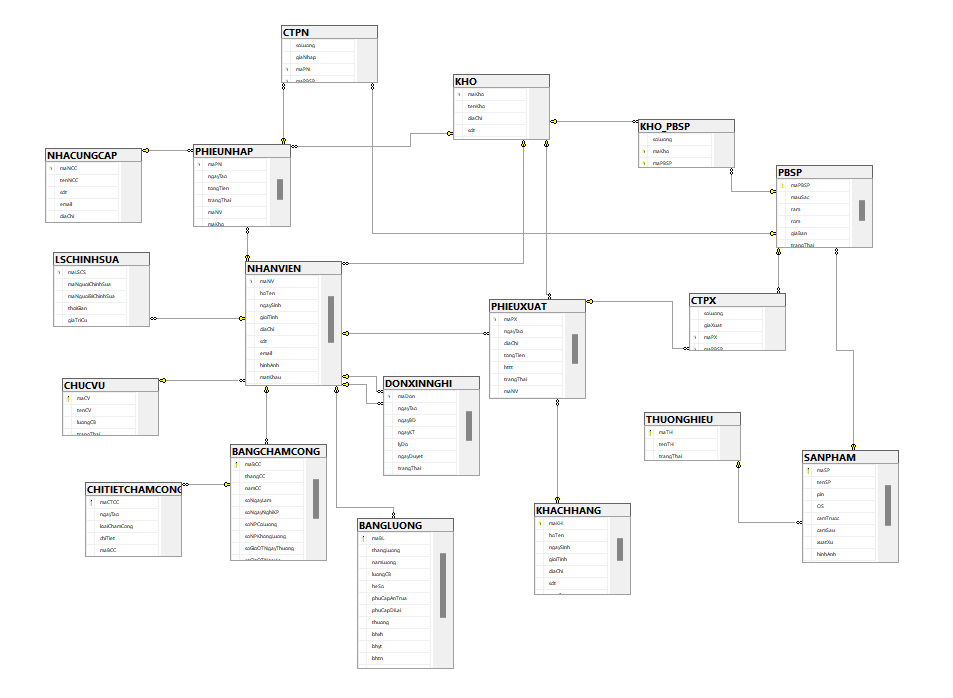
\includegraphics[width=0.9\linewidth]{../HTTDN/image/Bao-cao-HTTTDN/so-do-quan-he-dl.png}
    \caption{Sơ đồ quan hệ dữ liệu.}
    \label{fig:../HTTDN/image/Bao-cao-HTTTDN/so-do-quan-he-dl}
\end{figure}
BANGCHAMCONG (maBCC, thangCC, namCC, soNgayLam,\newline soNgayNghiKP, soNPCoLuong, soNPKhongLuong, soGioOTNgayThuong, soGioOTNgayLe, soGioOTCN, maNV)\\

BANGLUONG (maBL, thangLuong, namLuong, luongCB, heSo,\newline  phuCapAnTrua, phuCapDiLai, thuong, bhxh, bhyt, bhtn, thueTNCN, tamUng, thucNhan, maNV)\\

CHITIETCHAMCONG (maCTCC, ngayTao, loaiChamCong, chiTiet, maBCC, soGioOT)\\

CHUCVU (maCV, tenCV, luongCB, trangThai)\\

CTPN (maPN, maPBSP, soLuong, giaNhap)\\

CTPX (maPX, maPBSP, soLuong, giaXuat)\\

DONXINNGHI (maDon, ngayTao, ngayBD, ngayKT, lyDo, ngayDuyet, trangThai, maNV, maNguoiDuyet)\\

KHACHHANG (maKH, hoTen, ngaySinh, gioiTinh, diaChi, sdt, email, trangThai)\\

KHO (maKho, tenKho, diaChi, sdt, trangThai)\\

KHO\_PBSP (maKho, maPBSP, soLuong)\\

LSCHINHSUA (thoiGian, giaTriCu, giaTriMoi, maNguoiChinhSua,\newline maNguoiBiChinhSua)\\

NHACUNGCAP (maNCC, tenNCC, sdt, email, diaChi, trangThai)\\

NHANVIEN (maNV, hoTen, ngaySinh, gioiTinh, diaChi, sdt, email,\newline hinhAnh, matKhau, trangThai, maCV, chiNhanh)\\

PBSP (maPBSP, mauSac, ram, rom, giaBan, trangThai, maSP)\\

PHIEUNHAP (maPN, ngayTao, tongTien, trangThai, maNV, maKho, maNCC)\\

PHIEUXUAT (maPX, ngayTao, diaChi, tongTien, httt, trangThai, maNV, maKho, maKH)\\

SANPHAM (maSP, tenSP, pin, OS, camTruoc, camSau, xuatXu, hinhAnh, trangThai, maTH)\\

THUONGHIEU (maTH, tenTH, trangThai)\\

\section{Mô tả các bảng dữ liệu}
\subsection{Bảng THƯƠNG HIỆU}
\noindent
\begin{center}
    \begin{tabular}{|>{\centering\arraybackslash}p{3cm}|
        >{\centering\arraybackslash}p{4cm}|
        >{\centering\arraybackslash}p{4cm}|
        >{\centering\arraybackslash}p{4cm}|}
        \hline
        \textbf{Thuộc tính}                                                                                                               &
        \textbf{Kiểu dữ liệu}                                                                                                                             &
        \textbf{Ý nghĩa}                                                                                                 &
        \textbf{Ràng buộc}                                                                                                         \\
        \hline
        maTH &  VARCHAR(50)  & Mã thương hiệu & PRIMARY KEY, NOT NULL \\
        \hline
        tenTH &  NVARCHAR(255)  & Tên thương hiệu & NOT NULL \\                                                                                                                          
        \hline
        trangThai &  VARCHAR(10)  & Trạng thái hoạt~động & CHECK(‘on’, ‘off’), NOT NULL \\
        \hline
    \end{tabular}
\end{center}
\subsection{Bảng SẢN PHẨM}
\noindent
\begin{center}
    \begin{tabular}{|>{\centering\arraybackslash}p{3cm}|
        >{\centering\arraybackslash}p{4cm}|
        >{\centering\arraybackslash}p{4cm}|
        >{\centering\arraybackslash}p{4cm}|}
        \hline
        \textbf{Thuộc tính}                                                                                                               &
        \textbf{Kiểu dữ liệu}                                                                                                                             &
        \textbf{Ý nghĩa}                                                                                                 &
        \textbf{Ràng buộc}                                                                                                         \\
        \hline
        maSP &  VARCHAR(50)  & Mã sản phẩm & PRIMARY KEY, NOT NULL \\
        \hline
        tenSP &  NVARCHAR(255)  & Tên sản phẩm & NOT NULL \\
        \hline
        pin & NVARCHAR(50) & Dung lượng pin & NOT NULL \\                                                                                                                          
        \hline
        OS & NVARCHAR(50) & Hệ điều hành & NOT NULL \\                                                                                                                          
        \hline
        camTruoc & NVARCHAR(50) & Camera trước & NOT NULL \\                                                                                                                          
        \hline
        camSau & NVARCHAR(50) & Camera sau & NOT NULL \\                                                                                                                          
        \hline
        xuatXu & NVARCHAR(50) & Xuất xứ & NOT NULL \\                                                                                                                          
        \hline
        hinhAnh & NVARCHAR(50) & Hình ảnh (dạng BLOB) & NOT NULL \\                                                                                                                          
        \hline
        trangThai &  VARCHAR(10)  & Trạng thái sản~phẩm & CHECK(‘on’, ‘off’), NOT NULL \\
        \hline
        maTH & VARCHAR(50) & Mã thương hiệu & NOT NULL, FOREIGN KEY references THUONGHIEU \\                                                                                                                          
        \hline
    \end{tabular}
\end{center}
\subsection{Bảng PHIÊN BẢN SẢN PHẨM}
\noindent
\begin{center}
    \begin{longtable}{|>{\centering\arraybackslash}p{3cm}|
        >{\centering\arraybackslash}p{4cm}|
        >{\centering\arraybackslash}p{4cm}|
        >{\centering\arraybackslash}p{4cm}|}
        \hline
        \textbf{Thuộc tính}                                                                                                               &
        \textbf{Kiểu dữ liệu}                                                                                                                             &
        \textbf{Ý nghĩa}                                                                                                 &
        \textbf{Ràng buộc}                                                                                                         \\
        \hline
        maPBSP &  VARCHAR(50)  & Mã phiên bản sản phẩm & PRIMARY KEY, NOT NULL \\
        \hline
        mauSac &  NVARCHAR(50)  & Màu sắc & NOT NULL \\                                                                                                                          
        \hline
        ram & NVARCHAR(50) & Dung lượng RAM & NOT NULL \\                                                                                                                          
        \hline
        rom & NVARCHAR(50) & Dung lượng ROM & NOT NULL \\                                                                                                                          
        \hline
        giaBan & DECIMAL(18, 2) & Giá bán & NOT NULL \\                                                                                                                          
        \hline
        trangThai &  VARCHAR(10)  & Trạng thái phiên~bản & CHECK(‘on’, ‘off’), NOT NULL \\
        \hline
        maSP & VARCHAR(50) & Mã sản phẩm & NOT NULL, FOREIGN KEY references SANPHAM \\                                                                                                                          
        \hline
    \end{longtable}
\end{center}
\subsection{Bảng NHÀ CUNG CẤP}
\noindent
\begin{center}
    \begin{tabular}{|>{\centering\arraybackslash}p{3cm}|
        >{\centering\arraybackslash}p{4cm}|
        >{\centering\arraybackslash}p{4cm}|
        >{\centering\arraybackslash}p{4cm}|}
        \hline
        \textbf{Thuộc tính}                                                                                                               &
        \textbf{Kiểu dữ liệu}                                                                                                                             &
        \textbf{Ý nghĩa}                                                                                                 &
        \textbf{Ràng buộc}                                                                                                         \\
        \hline
        maNCC &  VARCHAR(50)  & Mã nhà cung cấp & PRIMARY KEY, NOT NULL \\
        \hline
        tenNCC &  NVARCHAR(255)  & Tên nhà cung cấp & NOT NULL \\                                                                                                                          
        \hline
        sdt & NVARCHAR(20) & Số điện thoại & NOT NULL \\                                                                                                                          
        \hline
        email & NVARCHAR(255) & Email &  \\                                                                                                                          
        \hline
        diaChi & NVARCHAR(255) & Địa chỉ & \\                                                                                                                          
        \hline
        trangThai &  VARCHAR(10)  & Trạng thái hoạt~động & CHECK(‘on’, ‘off’), NOT NULL \\
        \hline
    \end{tabular}
\end{center}
\subsection{Bảng CHỨC VỤ}
\noindent
\begin{center}
    \begin{tabular}{|>{\centering\arraybackslash}p{3cm}|
        >{\centering\arraybackslash}p{4cm}|
        >{\centering\arraybackslash}p{4cm}|
        >{\centering\arraybackslash}p{4cm}|}
        \hline
        \textbf{Thuộc tính}                                                                                                               &
        \textbf{Kiểu dữ liệu}                                                                                                                             &
        \textbf{Ý nghĩa}                                                                                                 &
        \textbf{Ràng buộc}                                                                                                         \\
        \hline
        maCV &  VARCHAR(50)  & Mã chức vụ & PRIMARY KEY, NOT NULL \\
        \hline
        tenCV &  NVARCHAR(255)  & Tên chức vụ & NOT NULL \\                                                                                                                          
        \hline
        luongCB & FLOAT & Lương cơ bản & NOT NULL \\                                                                                                                          
        \hline
        trangThai &  VARCHAR(50)  & Trạng thái hoạt~động & CHECK(‘on’, ‘off’), NOT NULL \\
        \hline
    \end{tabular}
\end{center}
\subsection{Bảng KHO}
\noindent
\begin{center}
    \begin{tabular}{|>{\centering\arraybackslash}p{3cm}|
        >{\centering\arraybackslash}p{4cm}|
        >{\centering\arraybackslash}p{4cm}|
        >{\centering\arraybackslash}p{4cm}|}
        \hline
        \textbf{Thuộc tính}                                                                                                               &
        \textbf{Kiểu dữ liệu}                                                                                                                             &
        \textbf{Ý nghĩa}                                                                                                 &
        \textbf{Ràng buộc}                                                                                                         \\
        \hline
        maKho &  VARCHAR(50)  & Mã kho & PRIMARY KEY, NOT NULL \\
        \hline
        tenKho &  NVARCHAR(255)  & Tên kho & NOT NULL \\                                                                                                                          
        \hline
        diaChi & NVARCHAR(255) & Địa chỉ kho & NOT NULL \\                                                                                                                          
        \hline
        sdt & VARCHAR(20) & Số điện thoại kho & NOT NULL \\                                                                                                                          
        \hline
        trangThai &  VARCHAR(10)  & Trạng thái hoạt~động & CHECK(‘on’, ‘off’), NOT NULL \\
        \hline
    \end{tabular}
\end{center}
\subsection{Bảng KHO\_PHIÊN BẢN SẢN PHẨM}
\noindent
\begin{center}
    \begin{tabular}{|>{\centering\arraybackslash}p{3cm}|
        >{\centering\arraybackslash}p{4cm}|
        >{\centering\arraybackslash}p{4cm}|
        >{\centering\arraybackslash}p{4cm}|}
        \hline
        \textbf{Thuộc tính}                                                                                                               &
        \textbf{Kiểu dữ liệu}                                                                                                                             &
        \textbf{Ý nghĩa}                                                                                                 &
        \textbf{Ràng buộc}                                                                                                         \\
        \hline
        soLuong &  INT  & Số lượng trong kho & NOT NULL \\
        \hline
        maKho &  VARCHAR(50)  & Mã kho & PRIMARY KEY (kết hợp), NOT~NULL, FOREIGN KEY references KHO \\                                                                                                                          
        \hline
        maPBSP &  VARCHAR(50)  & Mã phiên bản sản~phẩm & PRIMARY KEY (kết hợp), NOT~NULL, FOREIGN KEY references PBSP \\
        \hline
    \end{tabular}
\end{center}
\subsection{Bảng NHÂN VIÊN}
\noindent
\begin{center}
    \begin{longtable}{|>{\centering\arraybackslash}p{3cm}|
        >{\centering\arraybackslash}p{4cm}|
        >{\centering\arraybackslash}p{4cm}|
        >{\centering\arraybackslash}p{4cm}|}
        \hline
        \textbf{Thuộc tính}                                                                                                               &
        \textbf{Kiểu dữ liệu}                                                                                                                             &
        \textbf{Ý nghĩa}                                                                                                 &
        \textbf{Ràng buộc}                                                                                                         \\
        \hline
        maNV &  VARCHAR(50)  & Mã nhân viên & PRIMARY KEY, NOT NULL \\
        \hline
        hoTen &  NVARCHAR(255)  & Họ tên nhân viên & NOT NULL \\                                                                                                                          
        \hline
        ngaySinh & DATE & Ngày sinh & NOT NULL \\                                                                                                                          
        \hline
        gioiTinh & NVARCHAR(3) & Giới tính & CHECK(‘Nam’, ‘Nữ’), NOT NULL \\                                                                                                                          
        \hline
        diaChi & NVARCHAR(255) & Địa chỉ & NOT NULL \\                                                                                                                          
        \hline
        sdt & NVARCHAR(20) & Số điện thoại & NOT NULL \\                                                                                                                          
        \hline
        email & NVARCHAR(255) & Email & NOT NULL \\                                                                                                                          
        \hline
        hinhAnh & VARBINARY(MAX) & Hình ảnh & \\                                                                                                                          
        \hline
        matKhau & NVARCHAR(255) & Mật khẩu & NOT NULL \\                                                                                                                          
        \hline
        trangThai &  VARCHAR(10)  & Trạng thái hoạt~động & CHECK(‘on’, ‘off’), NOT NULL \\
        \hline
        maCV & VARCHAR(50) & Mã chức vụ & FOREIGN KEY references CHUCVU \\                                                                                                                          
        \hline
        chiNhanh & VARCHAR(50) & Mã kho (chi~nhánh) & FOREIGN KEY references KHO \\                                                                                                                          
        \hline
    \end{longtable}
\end{center}
\subsection{Bảng KHÁCH HÀNG}
\noindent
\begin{center}
    \begin{longtable}{|>{\centering\arraybackslash}p{3cm}|
        >{\centering\arraybackslash}p{4cm}|
        >{\centering\arraybackslash}p{4cm}|
        >{\centering\arraybackslash}p{4cm}|}
        \hline
        \textbf{Thuộc tính}                                                                                                               &
        \textbf{Kiểu dữ liệu}                                                                                                                             &
        \textbf{Ý nghĩa}                                                                                                 &
        \textbf{Ràng buộc}                                                                                                         \\
        \hline
        maKH &  VARCHAR(50)  & Mã khách hàng & PRIMARY KEY, NOT NULL \\
        \hline
        hoTen &  NVARCHAR(255)  & Họ tên khách hàng & NOT NULL \\                                                                                                                          
        \hline
        ngaySinh & DATE & Ngày sinhh & NOT NULL \\                                                                                                                          
        \hline
        gioiTinh & NVARCHAR(3) & Giới tính & CHECK(‘Nam’, ‘Nữ’), NOT NULL \\                                                                                                                          
        \hline
        diaChi & NVARCHAR(255) & Địa chỉ & NOT NULL \\                                                                                                                          
        \hline
        sdt & NVARCHAR(20) & Số điện thoại & NOT NULL \\                                                                                                                          
        \hline
        email & NVARCHAR(255) & Email & NOT NULL \\                                                                                                                          
        \hline
        trangThai &  VARCHAR(10)  & Trạng thái hoạt~động & CHECK(‘on’, ‘off’), NOT NULL \\
        \hline
    \end{longtable}
\end{center}
\subsection{Bảng PHIẾU NHẬP}
\noindent
\begin{center}
    \begin{tabular}{|>{\centering\arraybackslash}p{3cm}|
        >{\centering\arraybackslash}p{4cm}|
        >{\centering\arraybackslash}p{4cm}|
        >{\centering\arraybackslash}p{4cm}|}
        \hline
        \textbf{Thuộc tính}                                                                                                               &
        \textbf{Kiểu dữ liệu}                                                                                                                             &
        \textbf{Ý nghĩa}                                                                                                 &
        \textbf{Ràng buộc}                                                                                                         \\
        \hline
        maPN &  VARCHAR(50)  & Mã phiếu nhập & PRIMARY KEY, NOT NULL \\
        \hline
        ngayTao &  DATE  & Ngày tạo phiếu & NOT NULL \\                                                                                                                          
        \hline
        tongTien & FLOAT & Tổng tiền phiếu~nhập & \\                                                                                                                          
        \hline
        trangThai &  NVARCHAR(50)  & Trạng thái phiếu~nhập & CHECK(‘Chờ xác~nhận’, ‘Đã~xác~nhận’, ‘Đã~nhận~hàng’), NOT~NULL \\
        \hline
    \end{tabular}
\end{center}
\subsection{Bảng CHI TIẾT PHIẾU NHẬP}
\noindent
\begin{center}
    \begin{longtable}{|>{\centering\arraybackslash}p{3cm}|
        >{\centering\arraybackslash}p{4cm}|
        >{\centering\arraybackslash}p{4cm}|
        >{\centering\arraybackslash}p{4cm}|}
        \hline
        \textbf{Thuộc tính}                                                                                                               &
        \textbf{Kiểu dữ liệu}                                                                                                                             &
        \textbf{Ý nghĩa}                                                                                                 &
        \textbf{Ràng buộc}                                                                                                         \\
        \hline
        soLuong &  INT  & Số lượng sản phẩm nhập & NOT NULL \\
        \hline
        giaNhap &  DECIMAL(18, 2)  & Giá nhập & NOT NULL \\                                                                                                                          
        \hline
        maPN & VARCHAR(50) & Mã phiếu nhập & PRIMARY KEY (kết hợp), NOT~NULL, FOREIGN KEY references PHIEUNHAP \\                                                                                                                          
        \hline
        maPBSP &  VARCHAR(10)  & Mã phiên bản sản~phẩm & PRIMARY KEY (kết hợp), NOT~NULL, FOREIGN KEY references PBSP \\
        \hline
    \end{longtable}
\end{center}
\subsection{Bảng PHIẾU XUẤT}
\noindent
\begin{center}
    \begin{longtable}{|>{\centering\arraybackslash}p{3cm}|
        >{\centering\arraybackslash}p{4cm}|
        >{\centering\arraybackslash}p{4cm}|
        >{\centering\arraybackslash}p{4cm}|}
        \hline
        \textbf{Thuộc tính}                                                                                                               &
        \textbf{Kiểu dữ liệu}                                                                                                                             &
        \textbf{Ý nghĩa}                                                                                                 &
        \textbf{Ràng buộc}                                                                                                         \\
        \hline
        maPX &  VARCHAR(50)  & Mã phiếu xuất & PRIMARY KEY, NOT NULL \\
        \hline
        ngayTao & DATE  & Ngày tạo phiếu & NOT NULL \\                                                                                                                          
        \hline
        diaChi & NVARCHAR(255) & Địa chỉ giao hàng &  \\                                                                                                                          
        \hline
        tongTien & FLOAT & Tổng tiền phiếu xuất &  \\                                                                                                                          
        \hline
        httt & NVARCHAR(50) & Hình thức thanh toán & \\                                                                                                                          
        \hline
        trangThai &  NVARCHAR(50)  & Trạng thái phiếu~xuất & CHECK(‘Chờ xác~nhận’, ‘Đã xác~nhận’, ‘Đã xuất~hàng’), NOT~NULL \\
        \hline
        maNV & NVARCHAR(50) & Mã nhân viên xuất & NOT NULL, PRIMARY KEY (kết hợp), FOREIGN KEY references KHO \\                                                                                                                          
        \hline
        maKho & NVARCHAR(50) & Mã kho xuất~hàng & NOT NULL, FOREIGN KEY references KHO \\                                                                                                                          
        \hline
        maKH & NVARCHAR(50) & Mã khách hàng & NOT NULL, FOREIGN KEY references KHACHHANG \\                                                                                                                          
        \hline
    \end{longtable}
\end{center}
\subsection{Bảng CHI TIẾT PHIẾU XUẤT}
\noindent
\begin{center}
    \begin{tabular}{|>{\centering\arraybackslash}p{3cm}|
        >{\centering\arraybackslash}p{4cm}|
        >{\centering\arraybackslash}p{4cm}|
        >{\centering\arraybackslash}p{4cm}|}
        \hline
        \textbf{Thuộc tính}                                                                                                               &
        \textbf{Kiểu dữ liệu}                                                                                                                             &
        \textbf{Ý nghĩa}                                                                                                 &
        \textbf{Ràng buộc}                                                                                                         \\
        \hline
        soLuong &  INT  & Số lượng sản phẩm xuất & NOT NULL \\
        \hline
        giaXuat &  DECIMAL(18, 2)  & Giá xuất & NOT NULL \\                                                                                                                          
        \hline
        maPX &  VARCHAR(50)  & Mã phiếu xuất & PRIMARY KEY (kết hợp), NOT`NULL, FOREIGN KEY references PHIEUXUAT \\
        \hline
        maPBSP & VARCHAR(50) & Mã phiên bản sản phẩm & PRIMARY KEY (kết hợp), NOT~NULL, FOREIGN KEY references PBSP \\                                                                                                                          
        \hline
    \end{tabular}
\end{center}
\subsection{Bảng ĐƠN XIN NGHỈ}
\noindent
\begin{center}
    \begin{longtable}{|>{\centering\arraybackslash}p{3cm}|
        >{\centering\arraybackslash}p{4cm}|
        >{\centering\arraybackslash}p{4cm}|
        >{\centering\arraybackslash}p{4cm}|}
        \hline
        \textbf{Thuộc tính}                                                                                                               &
        \textbf{Kiểu dữ liệu}                                                                                                                             &
        \textbf{Ý nghĩa}                                                                                                 &
        \textbf{Ràng buộc}                                                                                                         \\
        \hline
        maDon &  VARCHAR(50)  & Mã đơn xin nghỉ & NOT NULL \\
        \hline
        ngayTao &  DATE  & Ngày tạo đơn & NOT NULL \\                                                                                                                          
        \hline
        ngayBD &  DATE  & Ngày bắt đầu nghỉ & NOT NULL \\                                                                                                                          
        \hline
        ngayKT &  DATE  & Ngày kết thúc nghỉ & \\                                                                                                                          
        \hline
        lyDo &  NVARCHAR(MAX)  & Lý do xin nghỉ & NOT NULL \\                                                                                                                          
        \hline
        ngayDuyet &  DATE  & Ngày duyệt đơn & \\                                                                                                                          
        \hline
        trangThai &  NVARCHAR(20)  & Trạng thái đơn & CHECK ('Chờ~duyệt', 'Đã~duyệt', 'Từ~chối'), NOT NULL \\
        \hline
        maNV &  VARCHAR(50)  & Mã nhân viên xin nghỉ & NOT NULL, FOREIGN KEY references NHANVIEN \\                                                                                                                          
        \hline
        maNguoiDuyet &  VARCHAR(50)  & Mã người duyệt & FOREIGN KEY references NHANVIEN \\                                                                                                                          
        \hline
    \end{longtable}
\end{center}
\subsection{Bảng LỊCH SỬ CHỈNH SỬA}
\noindent
\begin{center}
    \begin{longtable}{|>{\centering\arraybackslash}p{4.5cm}|
        >{\centering\arraybackslash}p{4.2cm}|
        >{\centering\arraybackslash}p{2.5cm}|
        >{\centering\arraybackslash}p{3.8cm}|}
        \hline
        \textbf{Thuộc tính}                                                                                                               &
        \textbf{Kiểu dữ liệu}                                                                                                                             &
        \textbf{Ý nghĩa}                                                                                                 &
        \textbf{Ràng buộc}                                                                                                         \\
        \hline
        maNguoiChinhSua &  VARCHAR(50)  & Mã người chỉnh sửa & FOREIGN KEY references NHANVIEN \\
        \hline
        maNguoiBiChinhSua &  VARCHAR(50)  & Mã người bị chỉnh sửa & FOREIGN KEY references NHANVIEN \\                                                                                                                          
        \hline
        thoiGian &  DATE  & Thời gian chỉnh sửa & NOT NULL \\                                                                                                                          
        \hline
        giaTriCu &  NVARCHAR(MAX)  & Giá trị cũ & NOT NULL\\                                                                                                                          
        \hline
        giaTriMoi & NVARCHAR(MAX)  & Giá trị mới & NOT NULL \\                                                                                                                          
        \hline
    \end{longtable}
\end{center}
\subsection{Bảng LƯƠNG}
\noindent
\begin{center}
    \begin{longtable}{|>{\centering\arraybackslash}p{4.5cm}|
        >{\centering\arraybackslash}p{3.5cm}|
        >{\centering\arraybackslash}p{3.5cm}|
        >{\centering\arraybackslash}p{4cm}|}
        \hline
        \textbf{Thuộc tính}                                                                                                               &
        \textbf{Kiểu dữ liệu}                                                                                                                             &
        \textbf{Ý nghĩa}                                                                                                 &
        \textbf{Ràng buộc}                                                                                                         \\
        \hline
        maBL &  VARCHAR(50)  & Mã bảng chấm công & PRIMARY KEY \\
        \hline
        thangCC &  INT  & Tháng chấm công & NOT NULL \\                                                                                                                          
        \hline
        namCC &  INT  & Năm chấm công & NOT NULL \\                                                                                                                          
        \hline
        soNgayLam &  FLOAT  & Số ngày làm & \\                                                                                                                          
        \hline
        soNgayNghiKP &  FLOAT  & Số ngày nghỉ không phép & \\                                                                                                                          
        \hline
        soNPCoLuong &  FLOAT  & Số ngày nghỉ phép có lương & \\                                                                                                                          
        \hline
        soNPKhongLuong &  FLOAT  & Số ngày nghỉ phép không lương & \\
        \hline
        soGioOTNgayThuong &  FLOAT  & Số giờ OT ngày thường & \\                                                                                                                          
        \hline
        soGioOTCN &  FLOAT  & Số giờ OT chủ nhật & \\                                                                                                                          
        \hline
        maNV &  VARCHAR(50)  & Mã nhân viên xin nghỉ & NOT NULL, FOREIGN KEY references NHANVIEN \\                                                                                                                          
        \hline
        soGioOTNgayLe &  FLOAT  & Số giờ OT ngày lễ & \\                                                                                                                          
        \hline
    \end{longtable}
\end{center}
\subsection{Bảng CHI TIẾT CHẤM CÔNG}
\noindent
\begin{center}
    \begin{longtable}{|>{\centering\arraybackslash}p{3cm}|
        >{\centering\arraybackslash}p{4cm}|
        >{\centering\arraybackslash}p{3.5cm}|
        >{\centering\arraybackslash}p{4.5cm}|}
        \hline
        \textbf{Thuộc tính}                                                                                                               &
        \textbf{Kiểu dữ liệu}                                                                                                                             &
        \textbf{Ý nghĩa}                                                                                                 &
        \textbf{Ràng buộc}                                                                                                         \\
        \hline
        maCTCC &  VARCHAR(50)  & Mã chi tiết chấm & PRIMARY KEY \\
        \hline
        ngayTao &  DATE  & Ngày tạo chi tiết & NOT NULL \\                                                                                                                          
        \hline
        loaiChamCong &  NVARCHAR(255)  & Loại chấm~công & CHECK ('Tăng ca ngày lễ', 'Tăng ca chủ nhật', 'Tăng ca ngày thường', 'Nghỉ phép có lương', 'Nghỉ phép không lương ', 'Nghỉ không phép'), NOT~NULL \\                                                                                                                          
        \hline
        chiTiet &  NVARCHAR(255)  & Chi tiết (lý do ...) & \\                                                                                                                          
        \hline
        maBCC &  VARCHAR(50)  & Mã bảng chấm công & FOREIGN KEY references BANGCHAMCONG \\                                                                                                                          
        \hline
        soGioOT &  FLOAT  & Số giờ OT & \\                                                                                                                          
        \hline
    \end{longtable}
\end{center}
\section{Lược đồ phân mảnh}
\subsection{Mô tả}
\begin{itemize}
    \item KHO: Phân mảnh ngang chính theo MAKHO (‘HN’, ‘DN’, ‘HCM’)
        \begin{itemize}[label=+]
            \item KHO\_PBSP: Phân mảnh ngang dẫn xuất theo KHO
            \item PHIEUNHAP: Phân mảnh ngang dẫn xuất theo KHO
                \begin{itemize}[label=+]
                    \item CTPN: Phân mảnh ngang dẫn xuất theo PHIEUNHAP
                \end{itemize}
            \item PHIEUXUAT: Phân mảnh ngang dẫn xuất theo KHO
                \begin{itemize}[label=+]
                    \item CTPX: Phân mảnh ngang dẫn xuất theo PHIEUXUAT
                \end{itemize}
            \item NHANVIEN: Phân mảnh ngang dẫn xuất theo KHO
                \begin{itemize}[label=+]
                    \item BANGLUONG: Phân mảnh ngang dẫn xuất theo NHANVIEN
                    \item BANGCHAMCONG: Phân mảnh ngang dẫn xuất theo NHANVIEN
                        \begin{itemize}[label=+]
                            \item CHITIETCHAMCONG: Phân mảnh ngang dẫn xuất theo \\ BANGCHAMCONG
                        \end{itemize}
                    \item DONXINNGHI: Phân mảnh ngang dẫn xuất theo NHANVIEN
                    \item LSCHINHSUA: Phân mảnh ngang dẫn xuất theo NHANVIEN
                \end{itemize}
            \item KHACHHANG: Phân mảnh ngang dẫn xuất theo KHO
        \end{itemize}
    \item THUONGHIEU, SANPHAM, CHUCVU, KHACHHANG,\newline NHACUNGCAP, PBSP: Nhân bản
\end{itemize}
\subsection{Biểu thức phân mảnh}
\subsubsection{Bảng KHO}
\begin{itemize}
    \item Quan hệ toàn cục: KHO (maKho, tenKho, diaChi,…)
    \item Phân mảnh ngang:
        \begin{itemize}[label=]
            \item \[KHO\_HN = \sigma_{maKho = 'HN'}(KHO)\]
            \item \[KHO\_DN = \sigma_{maKho = 'DN'}(KHO)\]
            \item \[KHO\_HCM = \sigma_{maKho = 'HCM'}(KHO)\]
        \end{itemize}
    \item Vị từ:
        \begin{itemize}[label=]
        \item \[Q_1\colon\quad maKho = 'HN'\]
        \item \[Q_2\colon\quad maKho = 'DN' \]
        \item \[Q_3\colon\quad maKho = 'HCM'\]
    \end{itemize}
\end{itemize}
\subsubsection{Bảng NHANVIEN}
\begin{itemize}
    \item Quan hệ toàn cục: NHANVIEN (maNV, hoTen, ngaySinh, \ldots)
    \item Phân mảnh ngang:
        \begin{itemize}[label=]
            \item \[NHANVIEN\_HN = NHANVIEN \bowtie_{chiNhanh = maKho}(KHO\_HN)\]
            \item \[NHANVIEN\_DN = NHANVIEN \bowtie_{chiNhanh = maKho}(KHO\_DN)\]
            \item \[NHANVIEN\_HCM = NHANVIEN \bowtie_{chiNhanh = maKho}(KHO\_HCM)\]
        \end{itemize}
    \item Vị từ:
    \begin{itemize}[label=]
        \item \[Q_4\colon\quad chiNhanh = maKho \quad and \quad Q_1\]
        \item \[Q_5\colon\quad chiNhanh = maKho \quad and \quad Q_2 \]
        \item \[Q_6\colon\quad chiNhanh = maKho \quad and \quad Q_3\]
    \end{itemize}
\end{itemize}
\subsubsection{Bảng PHIEUNHAP}
\begin{itemize}
    \item Quan hệ toàn cục: PHIEUNHAP (maPN, ngayTao, tongTien,  \ldots)
    \item Phân mảnh ngang:
        \begin{itemize}[label=]
            \item \[PHIEUNHAP\_HN = PHIEUNHAP \bowtie_{maKho}(KHO\_HN)\]
            \item \[PHIEUNHAP\_DN = PHIEUNHAP \bowtie_{maKho}(KHO\_DN)\]
            \item \[PHIEUNHAP\_HCM = PHIEUNHAP \bowtie_{maKho}(KHO\_HCM)\]
        \end{itemize}
    \item Vị từ:
    \begin{itemize}[label=]
        \item \[Q_7\colon\quad PHIEUNHAP.maKho = KHO\_HN.maKho \quad and \quad Q_1\]
        \item \[Q_8\colon\quad PHIEUNHAP.maKho = KHO\_DN.maKho \quad and \quad Q_2 \]
        \item \[Q_9\colon\quad PHIEUNHAP.maKho = KHO\_HCM.maKho \quad and \quad Q_3\]
    \end{itemize}
\end{itemize}
\subsubsection{Bảng PHIEUXUAT}
\begin{itemize}
    \item Quan hệ toàn cục: PHIEUXUAT (maPX, ngayTao, diaChi,  \ldots)
    \item Phân mảnh ngang:
        \begin{itemize}[label=]
            \item \[PHIEUXUAT\_HN = PHIEUXUAT \bowtie_{maKho}(KHO\_HN)\]
            \item \[PHIEUXUAT\_DN = PHIEUXUAT \bowtie_{maKho}(KHO\_DN)\]
            \item \[PHIEUXUAT\_HCM = PHIEUXUAT \bowtie_{maKho}(KHO\_HCM)\]
        \end{itemize}
    \item Vị từ:
    \begin{itemize}[label=]
        \item \[Q_10\colon\quad PHIEUXUAT.maKho = KHO\_HN.maKho \quad and \quad Q_1\]
        \item \[Q_11\colon\quad PHIEUXUAT.maKho = KHO\_DN.maKho \quad and \quad Q_2 \]
        \item \[Q_12\colon\quad PHIEUXUAT.maKho = KHO\_HCM.maKho \quad and \quad Q_3\]
    \end{itemize}
\end{itemize}
\subsubsection{Bảng LUONG}
\begin{itemize}
    \item Quan hệ toàn cục: \begin{itemize}
        \item Quan hệ toàn cục: BANGLUONG (maBL, thangLuong, namLuong,\ldots)
        \item Phân mảnh ngang:
            \begin{itemize}[label=]
                \item \[BANGLUONG\_HN = BANGLUONG \bowtie_{maNV}(NHANVIEN\_HN)\]
                \item \[BANGLUONG\_DN = BANGLUONG \bowtie_{maNV}(NHANVIEN\_DN)\]
                \item \[BANGLUONG\_HCM = BANGLUONG \bowtie_{maNV}(NHANVIEN\_HCM)\]
            \end{itemize}
        \item Vị từ:
        \begin{itemize}[label=]
            \item \[Q_{13}\colon\quad BANGLUONG.maNV = NHANVIEN\_HN.maNV \quad and \quad Q_4\]
            \item \[Q_{14}\colon\quad BANGLUONG.maNV = NHANVIEN\_DN.maNV \quad and \quad Q_5 \]
            \item \[Q_{15}\colon\quad BANGLUONG.maNV = NHANVIEN\_HCM.maNV \quad and \quad Q_6\]
        \end{itemize}
    \end{itemize}
\end{itemize}
\subsubsection{Bảng DONXINNGHI}
\begin{itemize}
    \item Quan hệ toàn cục: DONXINNGHI (maDon, ngayTao, ngayBD, \ldots)
    \item Phân mảnh ngang:
        \begin{itemize}[label=]
            \item \[DONXINNGHI\_HN = DONXINNGHI \bowtie_{maNV}(NHANVIEN\_HN)\]
            \item \[DONXINNGHI\_DN = DONXINNGHI \bowtie_{maNV}(NHANVIEN\_DN)\]
            \item \[DONXINNGHI\_HCM = DONXINNGHI \bowtie_{maNV}(NHANVIEN\_HCM)\]
        \end{itemize}
    \item Vị từ:
    \begin{itemize}[label=]
        \item \[Q_{16}\colon\quad BANGLUONG.maNV = NHANVIEN\_HN.maNV \quad and \quad Q_4\]
        \item \[Q_{17}\colon\quad BANGLUONG.maNV = NHANVIEN\_DN.maNV \quad and \quad Q_5 \]
        \item \[Q_{18}\colon\quad BANGLUONG.maNV = NHANVIEN\_HCM.maNV \quad and \quad Q_6\]
    \end{itemize}
\end{itemize}
\subsubsection{Bảng LSCHINHSUA}
\begin{itemize}
    \item Quan hệ toàn cục: LSCHINHSUA (maNguoiChinhSua, maNguoiBiChinhSua, \ldots)
    \item Phân mảnh ngang:
        \begin{itemize}[label=]
            \item \[LSCHINHSUA\_HN = LSCHINHSUA \bowtie_{maNguoiBiChinhSua=maNV}(NHANVIEN\_HN)\]
            \item \[LSCHINHSUA\_DN = LSCHINHSUA \bowtie_{maNguoiBiChinhSua=maNV}(NHANVIEN\_DN)\]
            \item \[LSCHINHSUA\_HCM = LSCHINHSUA \bowtie_{maNguoiBiChinhSua=maNV}(NHANVIEN\_HCM)\]
        \end{itemize}
    \item Vị từ:
    \begin{itemize}[label=]
        \item \[Q_{19}\colon\quad LSCHINHSUA.maNguoiBiChinhSua = NHANVIEN\_HN.maNV \quad and \quad Q_4\]
        \item \[Q_{20}\colon\quad LSCHINHSUA.maNguoiBiChinhSua = NHANVIEN\_DN.maNV \quad and \quad Q_5 \]
        \item \[Q_{21}\colon\quad LSCHINHSUA.maNguoiBiChinhSua = NHANVIEN\_HCM.maNV \quad and \quad Q_6\]
    \end{itemize}
\end{itemize}
\subsubsection{Bảng BANGCHAMCONG}
\begin{itemize}
    \item Quan hệ toàn cục: BANGCHAMCONG (maBCC, thangCC, namCC, \ldots)
    \item Phân mảnh ngang:
        \begin{itemize}[label=]
            \item \[BANGCHAMCONG\_HN = BANGCHAMCONG \bowtie_{maNV}(NHANVIEN\_HN)\]
            \item \[BANGCHAMCONG\_DN = BANGCHAMCONG \bowtie_{maNV}(NHANVIEN\_DN)\]
            \item \[BANGCHAMCONG\_HCM = BANGCHAMCONG \bowtie_{maNV}(NHANVIEN\_HCM)\]
        \end{itemize}
    \item Vị từ:
    \begin{itemize}[label=]
        \item \[Q_{22}\colon\quad BANGCHAMCONG.maNV = NHANVIEN\_HN.maNV \quad and \quad Q_4\]
        \item \[Q_{23}\colon\quad BANGCHAMCONG.maNV = NHANVIEN\_DN.maNV \quad and \quad Q_5 \]
        \item \[Q_{24}\colon\quad BANGCHAMCONG.maNV = NHANVIEN\_HCM.maNV \quad and \quad Q_6\]
    \end{itemize}
\end{itemize}
\subsubsection{Bảng CHITIETCHAMCONG}
\begin{itemize}
    \item Quan hệ toàn cục:  CHITIETCHAMCONG (maCTCC, ngayTao, loaiChamCong, \ldots)
    \item Phân mảnh ngang:
        \begin{itemize}[label=]
            \item \[CHITIETCHAMCONG\_HN = CHITIETCHAMCONG \bowtie_{maBCC}(BANGCHAMCONG\_HN)\]
            \item \[CHITIETCHAMCONG\_DN = CHITIETCHAMCONG \bowtie_{maBCC}(BANGCHAMCONG\_DN)\]
            \item \[CHITIETCHAMCONG\_HCM = CHITIETCHAMCONG \bowtie_{maBCC}(BANGCHAMCONG\_HCM)\]
        \end{itemize}
    \item Vị từ:
    \begin{itemize}[label=]
        \item \[Q_{25}\colon\quad CHITIETCHAMCONG.maBCC = BANGCHAMCONG\_HN.maBCC \quad and \quad Q_{22}\]
        \item \[Q_{26}\colon\quad CHITIETCHAMCONG.maBCC = BANGCHAMCONG\_DN.maBCC \quad and \quad Q_{23} \]
        \item \[Q_{27}\colon\quad CHITIETCHAMCONG.maBCC = BANGCHAMCONG\_HCM.maBCC \quad and \quad Q_{24}\]
    \end{itemize}
\end{itemize}
\subsubsection{Bảng KHO\_PBSP}
\begin{itemize}
    \item Quan hệ toàn cục: KHO\_PBSP (maKho, maPBSP, soLuong)
    \item Phân mảnh ngang:
        \begin{itemize}[label=]
            \item \[KHO\_PBSP\_HN = KHO\_PBSP \bowtie_{maKho}(KHO\_HN)\]
            \item \[KHO\_PBSP\_DN = KHO\_PBSP \bowtie_{maKho}(KHO\_DN)\]
            \item \[KHO\_PBSP\_HCM = KHO\_PBSP \bowtie_{maKho}(KHO\_HCM)\]
        \end{itemize}
    \item Vị từ:
    \begin{itemize}[label=]
        \item \[Q_{28}\colon\quad KHO\_PBSP.maKho = KHO\_HN.maKho \quad and \quad Q_1\]
        \item \[Q_{29}\colon\quad KHO\_PBSP.maKho = KHO\_DN.maKho \quad and \quad Q_2 \]
        \item \[Q_{30}\colon\quad KHO\_PBSP.maKho = KHO\_HCM.maKho \quad and \quad Q_3\]
    \end{itemize}
\end{itemize}
\subsubsection{Bảng CTPN}
\begin{itemize}
    \item Quan hệ toàn cục: CTPN (maPN, maPBSP, soLuong, \ldots)
    \item Phân mảnh ngang:
        \begin{itemize}[label=]
            \item \[CTPN\_HN = CTPN \bowtie_{maPN}(PHIEUNHAP\_HN)\]
            \item \[CTPN\_DN = CTPN \bowtie_{maPN}(PHIEUNHAP\_DN)\]
            \item \[CTPN\_HCM = CTPN \bowtie_{maPN}(PHIEUNHAP\_HCM)\]
        \end{itemize}
    \item Vị từ:
    \begin{itemize}[label=]
        \item \[Q_{31}\colon\quad CTPN.maPN = PHIEUNHAP\_HN.maPN \quad and \quad Q_7\]
        \item \[Q_{32}\colon\quad CTPN.maPN = PHIEUNHAP\_DN.maPN \quad and \quad Q_8 \]
        \item \[Q_{33}\colon\quad CTPN.maPN = PHIEUNHAP\_HCM.maPN \quad and \quad Q_9\]
    \end{itemize}
\end{itemize}
\subsubsection{Bảng CTPX}
\begin{itemize}
    \item Quan hệ toàn cục: CTPX (maPX, maPBSP, soLuong,  \ldots)
    \item Phân mảnh ngang:
        \begin{itemize}[label=]
            \item \[CTPX\_HN = CTPX \bowtie_{maPX}(PHIEUXUAT\_HN)\]
            \item \[CTPX\_DN = CTPX \bowtie_{maPX}(PHIEUXUAT\_DN)\]
            \item \[CTPX\_HCM = CTPX \bowtie_{maPX}(PHIEUXUAT\_HCM)\]
        \end{itemize}
    \item Vị từ:
    \begin{itemize}[label=]
        \item \[Q_{34}\colon\quad CTPX.maPX = PHIEUXUAT\_HN.maPX \quad and \quad Q_{10}\]
        \item \[Q_{35}\colon\quad CTPX.maPX = PHIEUXUAT\_DN.maPX \quad and \quad Q_{11} \]
        \item \[Q_{36}\colon\quad CTPX.maPX = PHIEUXUAT\_HCM.maPX \quad and \quad Q_{12}\]
    \end{itemize}
\end{itemize}
\chapter{CÀI ĐẶT VÀ TRUY VẤN CƠ SỞ DỮ LIỆU PHÂN TÁN}
\section{Cài đặt cơ sở dữ liệu phân tán}
\subsection{Chuẩn bị}
    \begin{itemize}
        \item Ta tạo 1 folder D:\textbackslash ReplData để chứa các dữ liệu trao đổi trong quá trình update dữ liệu từ các phân mảnh về cơ sở dữ liệu gốc, và từ cơ sở dữ liệu gốc đến các phân mảnh.
        \item Tiến hành cho folder này là 1 snapshot folder: thực chất là 1 shared folder trong Windows, cho phép các users được quyền read/write.
        \item Right click trên folder REPLDATA, chọn Properties, chọn tab Sharing – Share.
    \end{itemize}
    \begin{figure}[H]
        \centering
        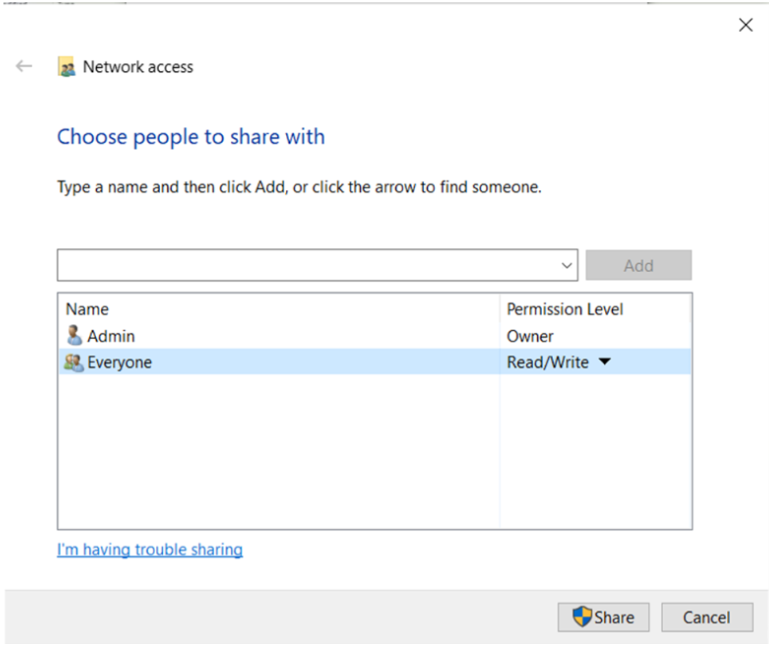
\includegraphics[width=0.45\linewidth]{img/01.png} \hfill
        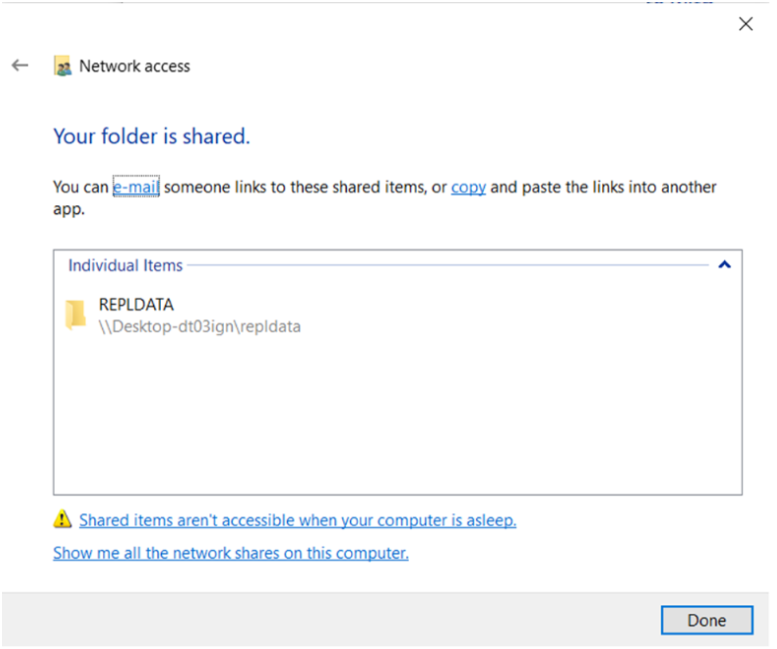
\includegraphics[width=0.45\linewidth]{img/1.png} \\
        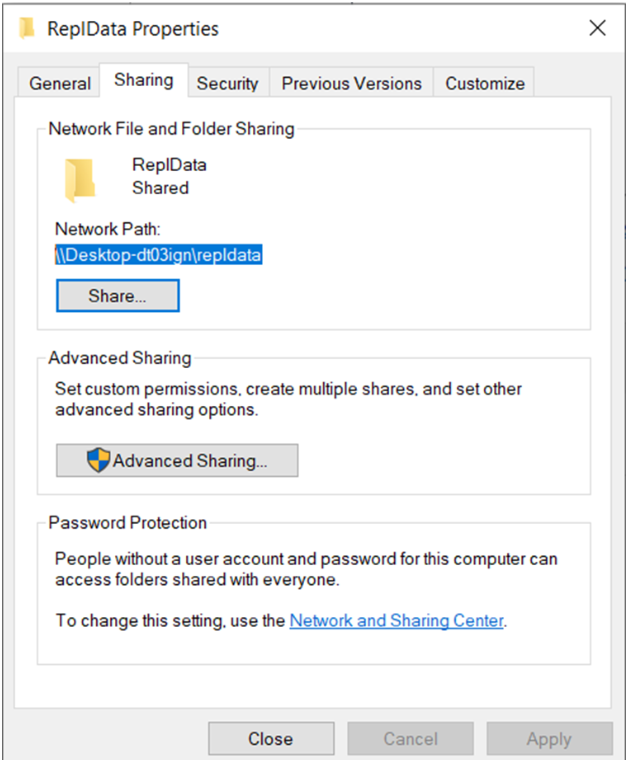
\includegraphics[width=0.5\linewidth]{img/2.png}
    \end{figure}
    \begin{enumerate}[label=Bước \arabic*:]
        \item Configure Distribution "Mở SQL Server, chọn server \textbackslash HUYHNK1 là Distributor và Pulisher (server gốc)"
        \begin{figure}[H]
            \centering
            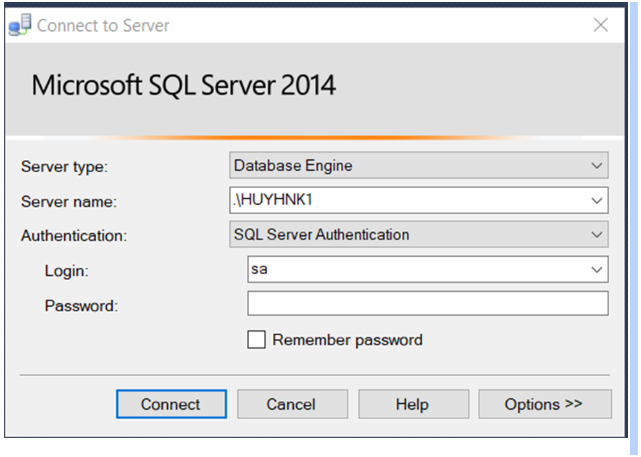
\includegraphics[width=0.5\linewidth]{img/3.png}
        \end{figure}
        \item Right click và Replication:
        \begin{figure}[H]
            \centering
            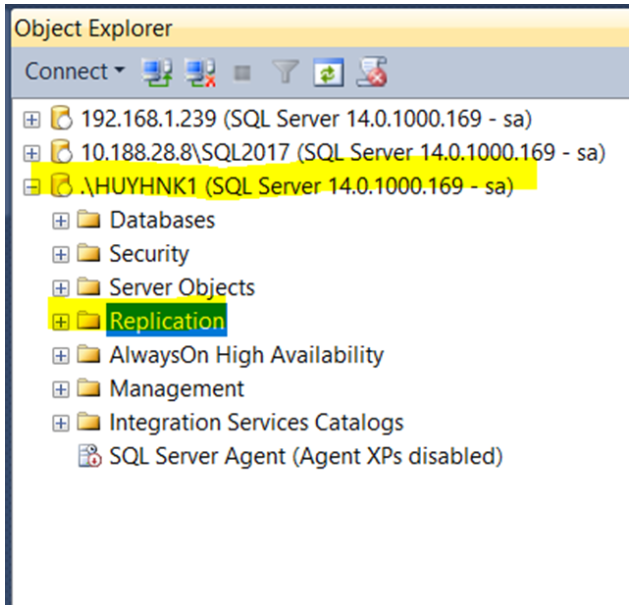
\includegraphics[width=0.5\linewidth]{img/4.png} \hfill
            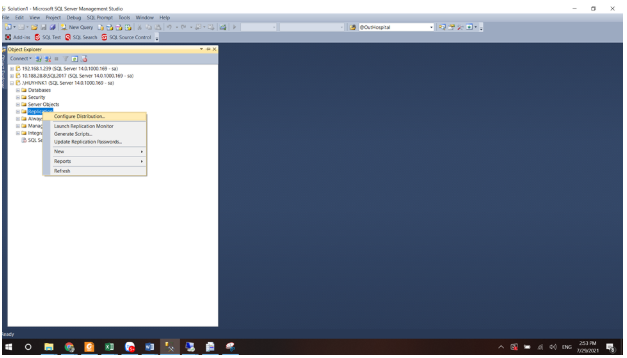
\includegraphics[width=0.5\linewidth]{img/5.png}
        \end{figure}
        \item Chọn Config Distribution
        \begin{figure}[H]
            \centering
            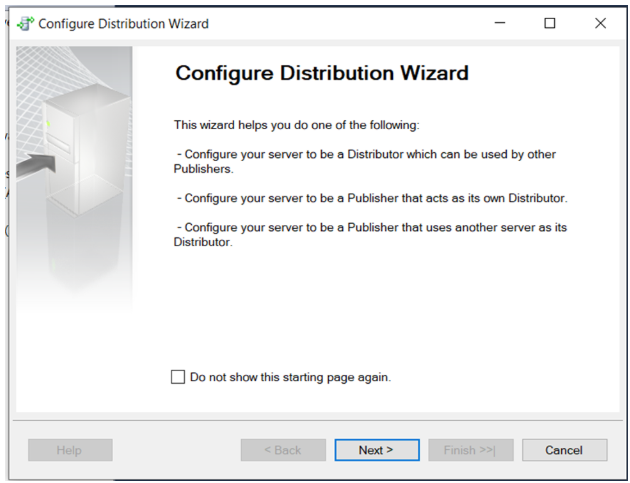
\includegraphics[width=0.5\linewidth]{img/6.png}
        \end{figure}
        \item Chọn next
        \begin{figure}[H]
            \centering
            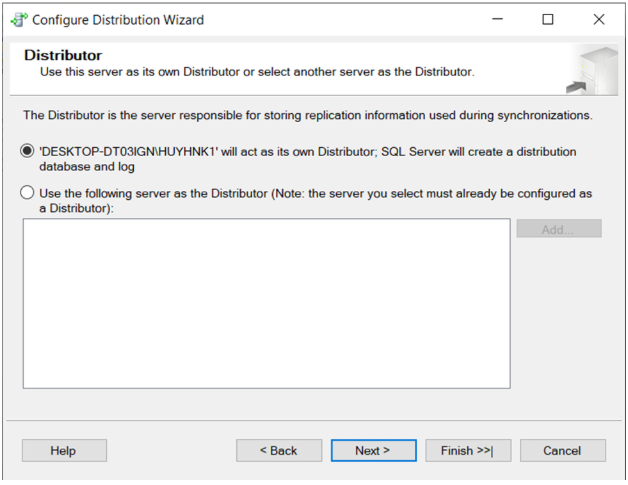
\includegraphics[width=0.5\linewidth]{img/7.png}
        \end{figure}
        \item Next
        \begin{figure}[H]
            \centering
            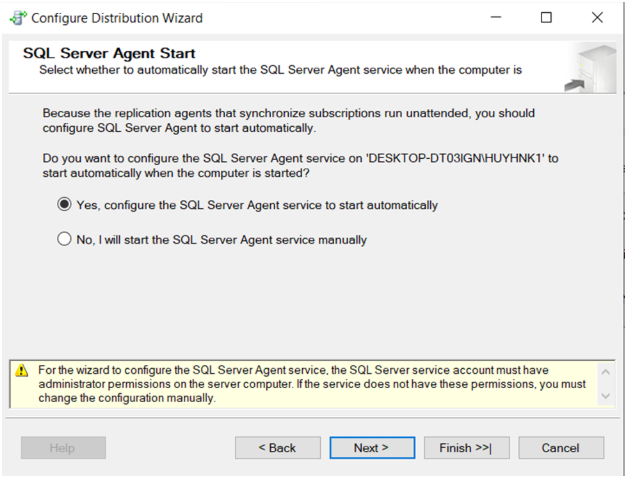
\includegraphics[width=0.5\linewidth]{img/8.png}
        \end{figure}
        \item Next
        \begin{figure}[H]
            \centering
            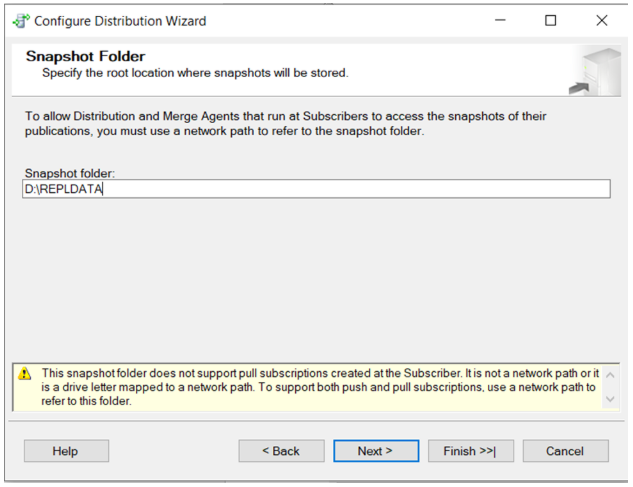
\includegraphics[width=0.5\linewidth]{img/9.png}
        \end{figure}
        \item Copy Đường dẫn Snapshot Folder vừa tạo ở bước trước \textbf{D:\textbackslash REPLDATA}
        \begin{figure}[H]
            \centering
            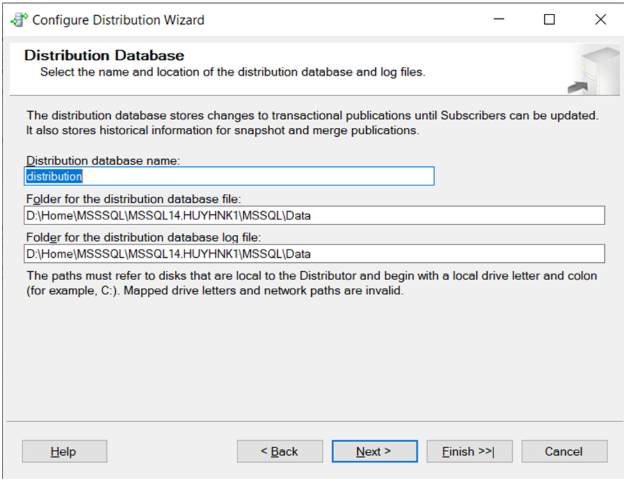
\includegraphics[width=0.5\linewidth]{img/10.png}
        \end{figure}
        \item Distribution là tên database chứa các metadata và các lịch sử data của các bản nhân (repication) và các giao tác.
        \begin{figure}[H]
            \centering
            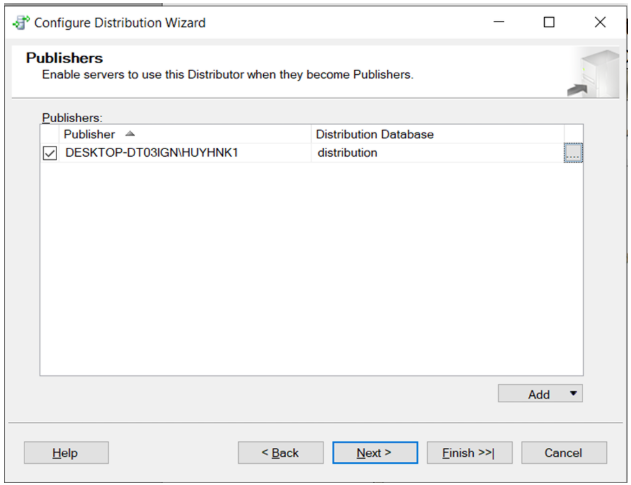
\includegraphics[width=0.5\linewidth]{img/11.png}
        \end{figure}
        \item Chọn Next
        \begin{figure}[H]
            \centering
            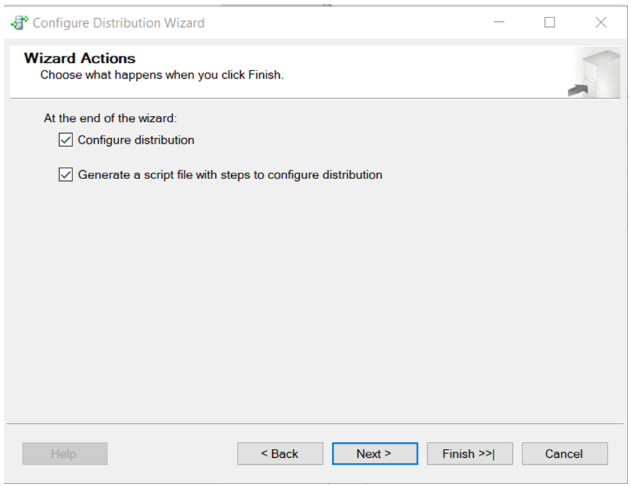
\includegraphics[width=0.5\linewidth]{img/12.png}
        \end{figure}
        \item Check chọn thêm vào Generate Script
        \begin{figure}[H]
            \centering
            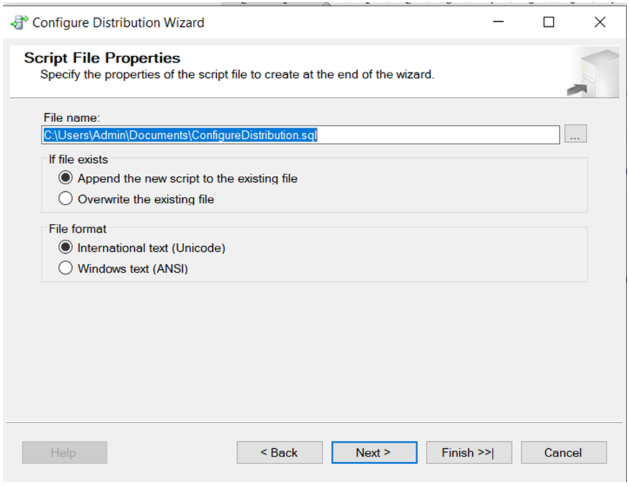
\includegraphics[width=0.5\linewidth]{img/13.png}
        \end{figure}
        \item Đường dẫn lưu script
        \begin{figure}[H]
            \centering
            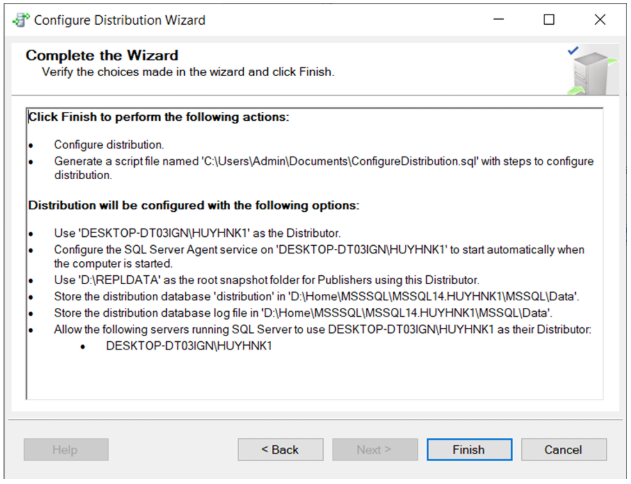
\includegraphics[width=0.5\linewidth]{img/14.png}
        \end{figure}
        \item Finish
        \begin{figure}[H]
            \centering
            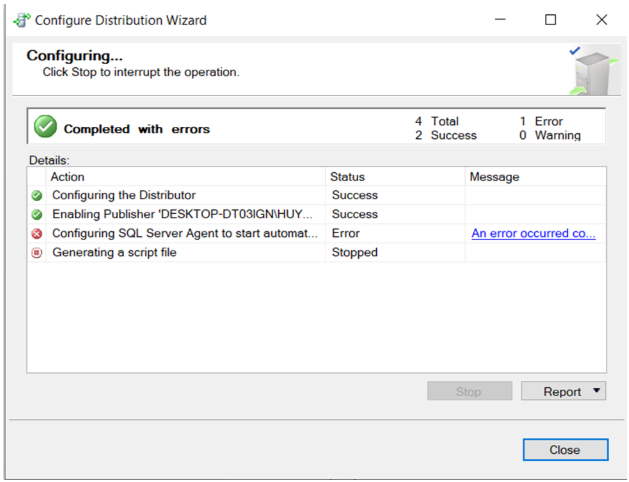
\includegraphics[width=0.5\linewidth]{img/15.png}
            \caption{Có thể có lỗi (như không quan trọng)}
        \end{figure}
        \item Start SQL server Agent lên
        \begin{figure}[H]
            \centering
            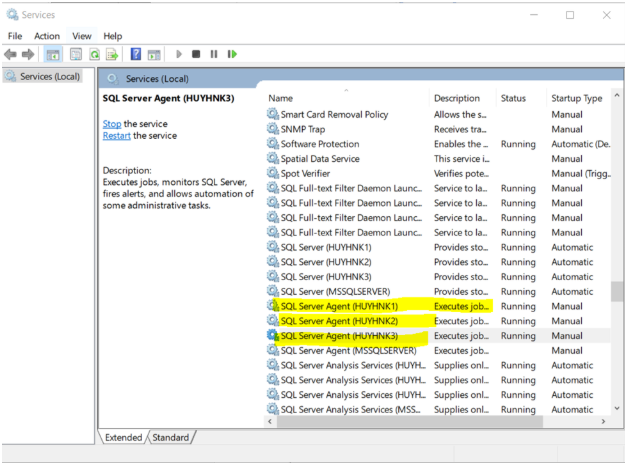
\includegraphics[width=0.5\linewidth]{img/16.png} \hfill
            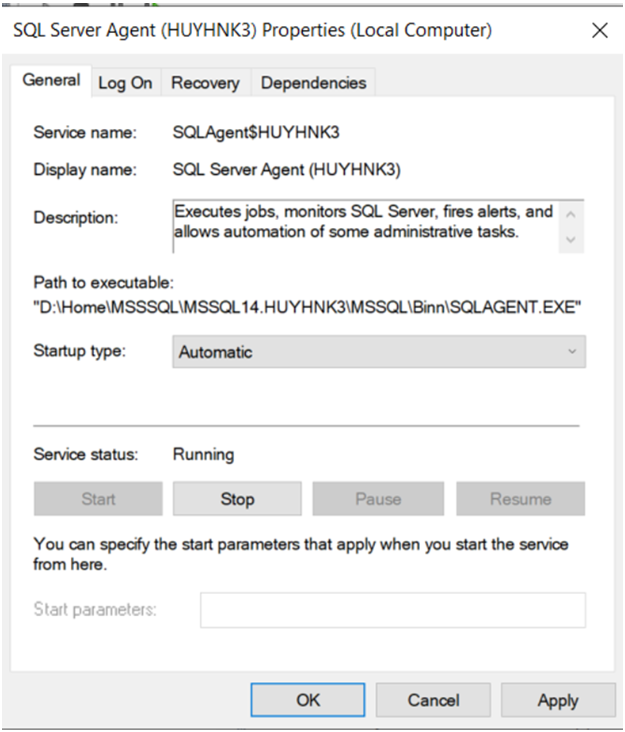
\includegraphics[width=0.5\linewidth]{img/17.png}
        \end{figure}
        \item Chọn startup type: Automatic. Để Disable server Distributor và Publisher
        \begin{figure}[H]
            \centering
            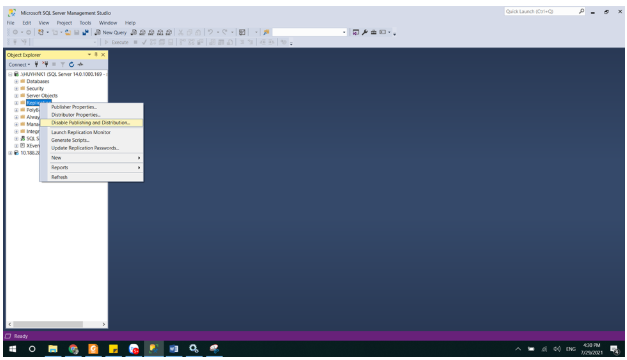
\includegraphics[width=0.5\linewidth]{img/18.png} \hfill
            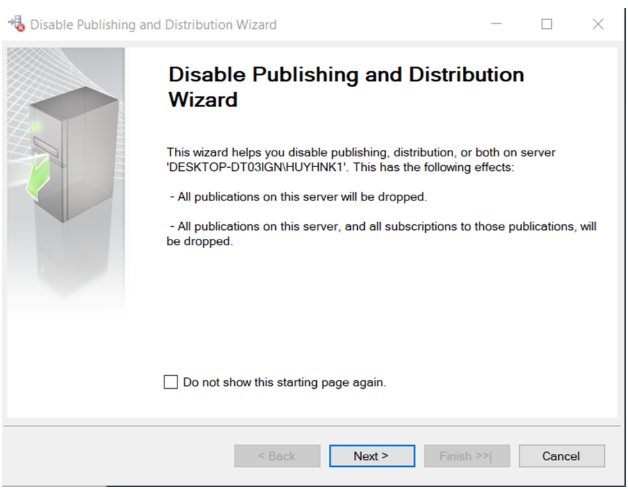
\includegraphics[width=0.5\linewidth]{img/19.png}
        \end{figure}
        \item Chọn Next
        \begin{figure}[H]
            \centering
            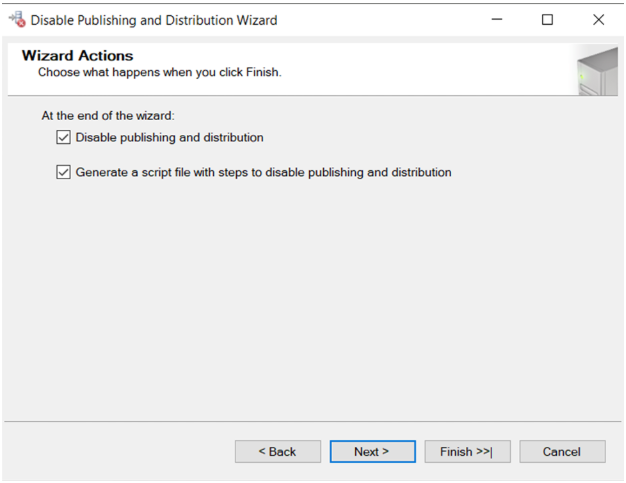
\includegraphics[width=0.5\linewidth]{img/20.png} \hfill
            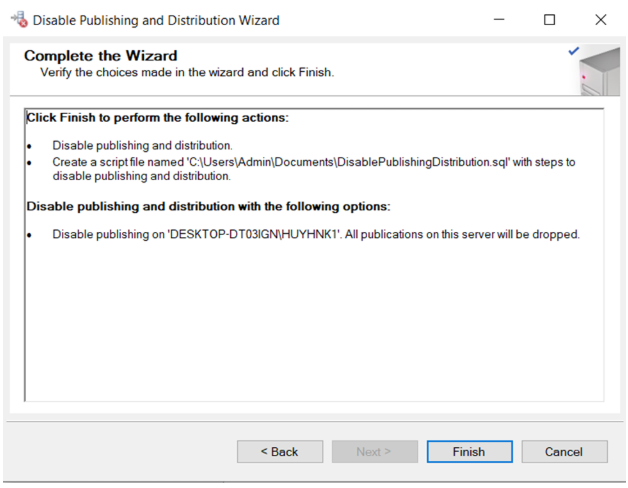
\includegraphics[width=0.5\linewidth]{img/21.png}
        \end{figure}
        \item Finish
    \end{enumerate}
\subsection{Cài đặt Publication }
\begin{enumerate}[label=Bước \arabic*:]
    \begin{figure}[H]
        \centering
        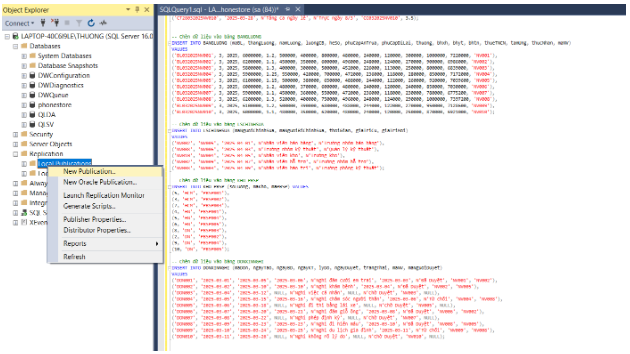
\includegraphics[width=0.5\linewidth]{img/22.png}
    \end{figure}
    \item Tạo Publication ở Server gốc
    \begin{figure}[H]
        \centering
        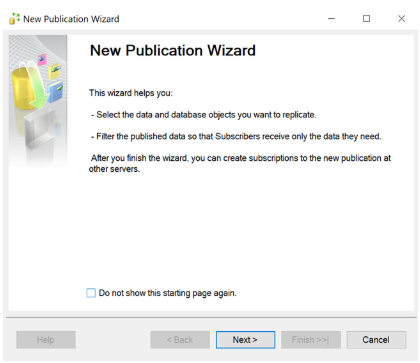
\includegraphics[width=0.5\linewidth]{img/23.png}
    \end{figure}
    \item Next
    \begin{figure}[H]
        \centering
        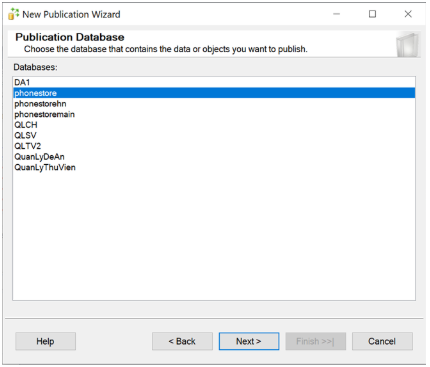
\includegraphics[width=0.5\linewidth]{img/24.png}
    \end{figure}
    \item Chọn CSDL cần phân tán dữ liệu: phonestore
    \begin{figure}[H]
        \centering
        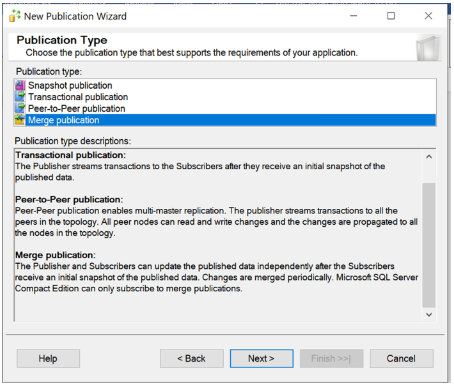
\includegraphics[width=0.5\linewidth]{img/25.png}
    \end{figure}
    \item Chọn Merge publication
    \begin{figure}[H]
        \centering
        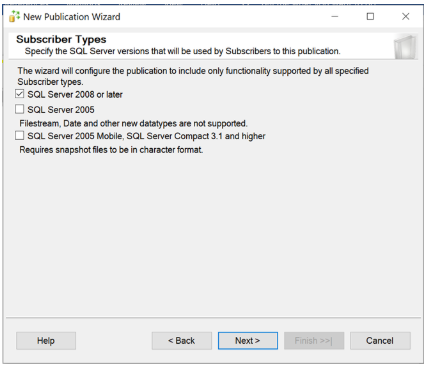
\includegraphics[width=0.5\linewidth]{img/26.png}
    \end{figure}
    \item Chọn bản phù hợp (mới nhất)
    \begin{figure}[H]
        \centering
        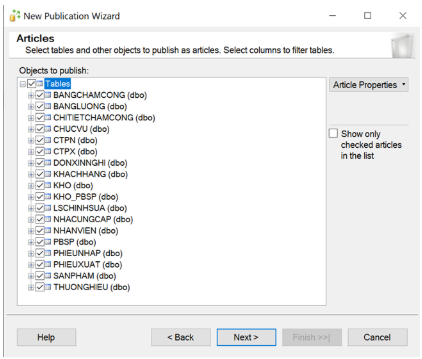
\includegraphics[width=0.5\linewidth]{img/27.png}
    \end{figure}
    \item Lựa chọn phân tán theo Table
    \begin{figure}[H]
        \centering
        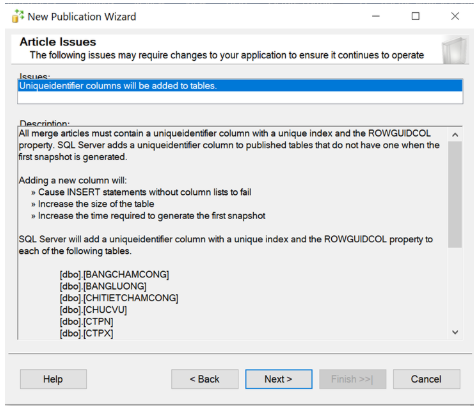
\includegraphics[width=0.5\linewidth]{img/28.png} \hfill
        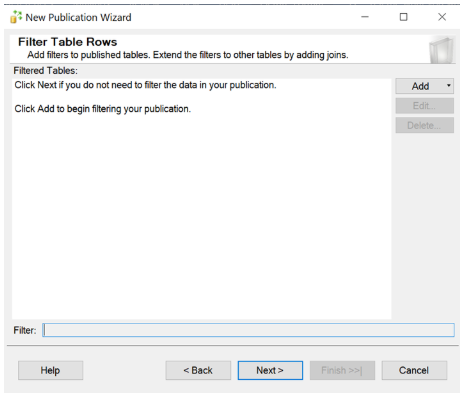
\includegraphics[width=0.5\linewidth]{img/29.png}
    \end{figure}
    \item Sau khi next hiện tiếp cửa sổ trên và chọn vào ADD
    \begin{figure}[H]
        \centering
        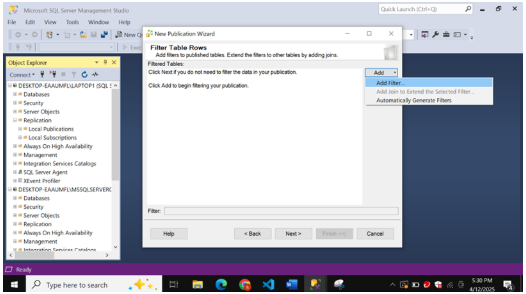
\includegraphics[width=0.5\linewidth]{img/30.png}
    \end{figure}
    \item Sau khi chọn vào Add filter
    \begin{figure}[H]
        \centering
        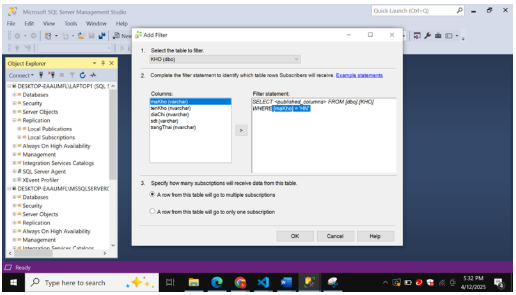
\includegraphics[width=0.5\linewidth]{img/31.png}
        \caption{\centering Chỗ select the table to filter tìm đến bảng kho do đang thực hiện phân tán theo kho}
    \end{figure}
    \item Sau đó chọn OK
    \begin{figure}[H]
        \centering
        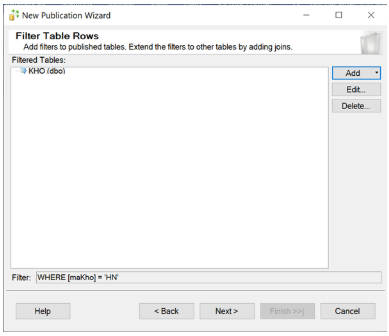
\includegraphics[width=0.5\linewidth]{img/32.png} \hfill
        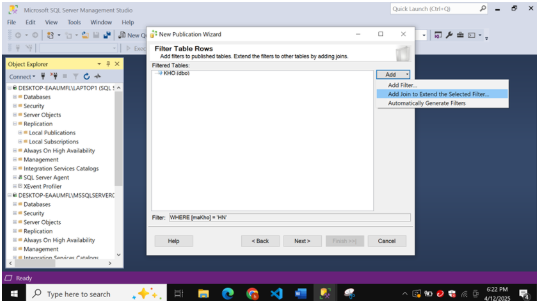
\includegraphics[width=0.5\linewidth]{img/33.png}
    \end{figure}
    \item Tiếp theo click vào add Join to extend dưới add filter để thực hiện phân tán.
    \begin{figure}[H]
        \centering
        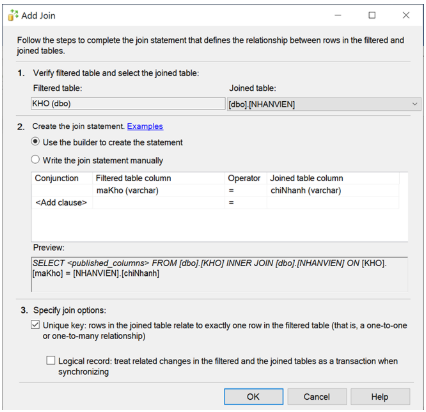
\includegraphics[width=0.5\linewidth]{img/34.png} \hfill
        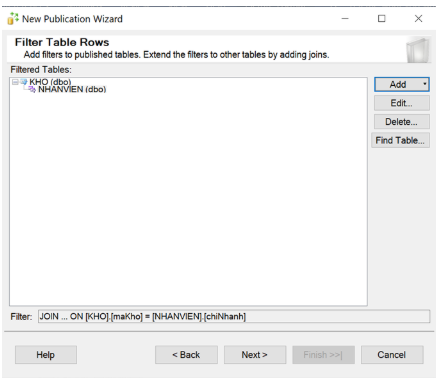
\includegraphics[width=0.5\linewidth]{img/35.png} \\
    \end{figure}
    \begin{figure}[H]
        \centering
        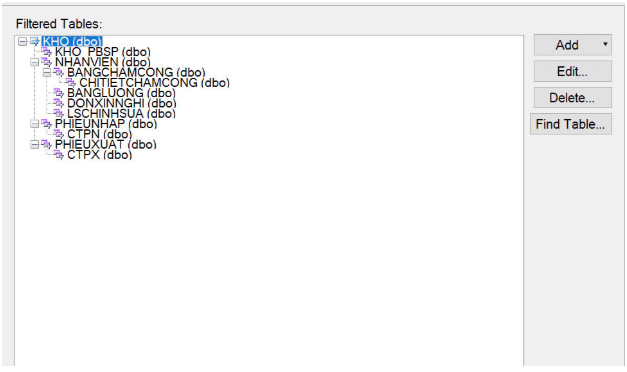
\includegraphics[width=0.5\linewidth]{img/36.png} \hfill
        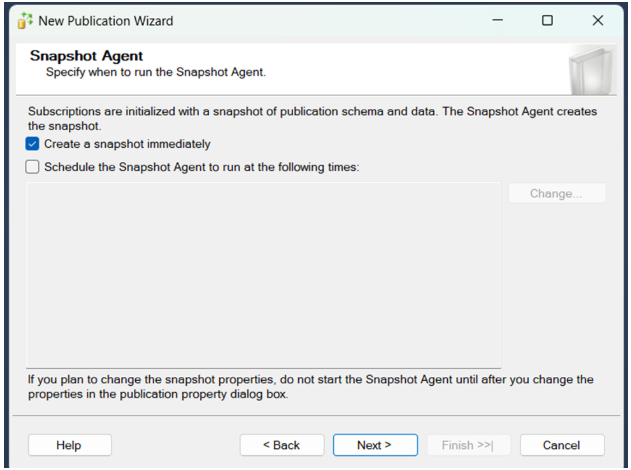
\includegraphics[width=0.5\linewidth]{img/37.png}
    \end{figure}
    \begin{figure}[H]
        \centering
        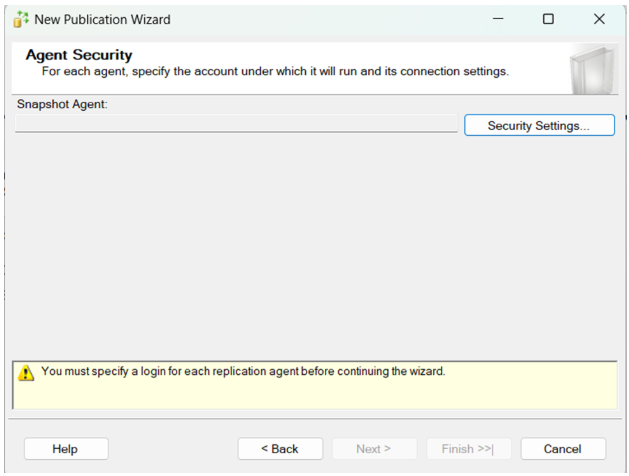
\includegraphics[width=0.5\linewidth]{img/38.png}
    \end{figure}
    \item Click vào security setting
    \begin{figure}[H]
        \centering
        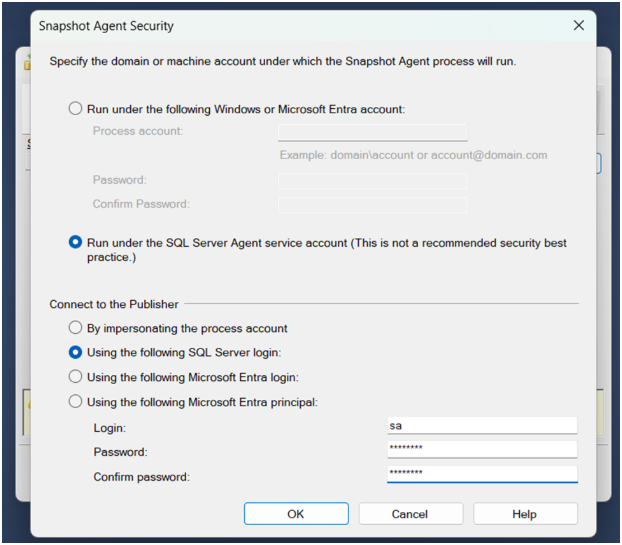
\includegraphics[width=0.5\linewidth]{img/39.png} \hfill
        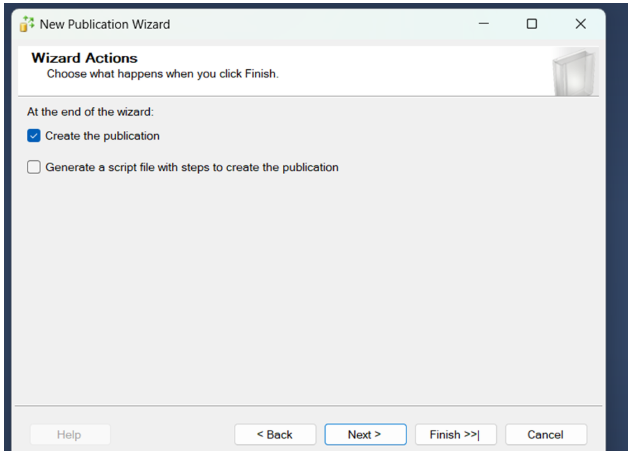
\includegraphics[width=0.5\linewidth]{img/40.png}
    \end{figure}
    \begin{figure}[H]
        \centering
        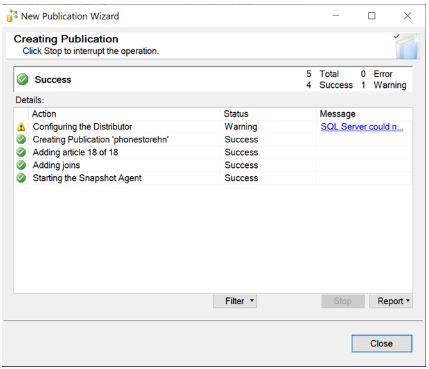
\includegraphics[width=0.5\linewidth]{img/41.png}\hfill
        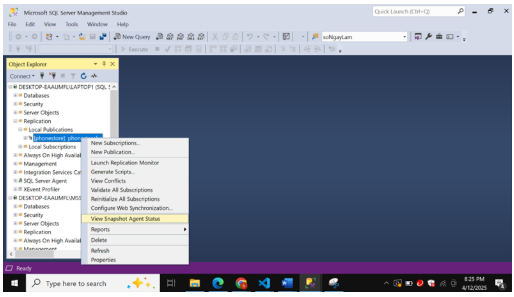
\includegraphics[width=0.5\linewidth]{img/42.png} 
    \end{figure}
    \begin{figure}[H]
        \centering
        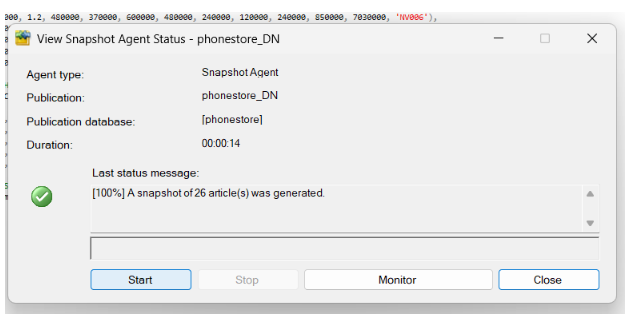
\includegraphics[width=0.5\linewidth]{img/43.png}
        \caption{Màn hình hiển thị thành công}
    \end{figure}
\end{enumerate}
\subsection{Cài đặt Subscription}
\subsubsection{Tạo server}
Chọn sql2022 -> DeveloperENU -> setup

\textbf{Thực hiện setup một server:}
\begin{figure}[H]
    \centering
    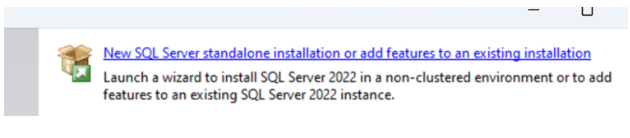
\includegraphics[width=0.5\linewidth]{img/44.png}
\end{figure}
\quad Chọn Installation
\begin{figure}[H]
    \centering
    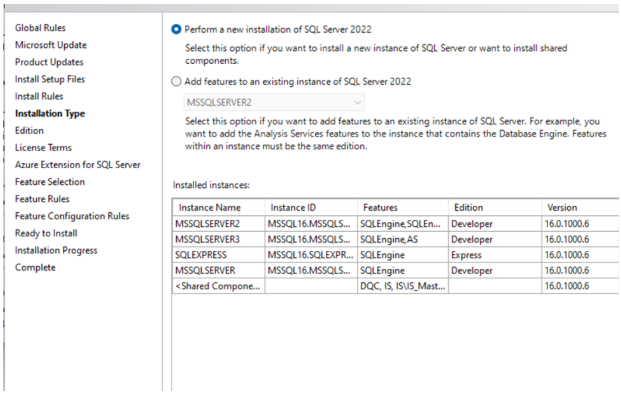
\includegraphics[width=0.5\linewidth]{img/45.png}
\end{figure}
\quad Chọn perform a new để tạo mới
\begin{figure}[H]
    \centering
    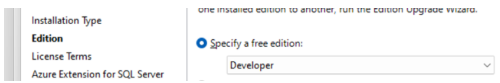
\includegraphics[width=0.5\linewidth]{img/46.png}
\end{figure}
\quad Edition:
\begin{figure}[H]
    \centering
    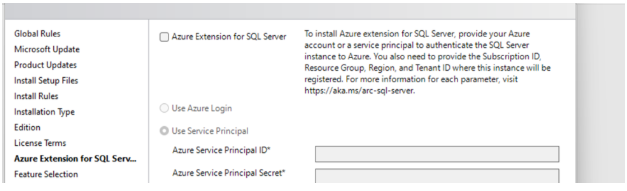
\includegraphics[width=0.5\linewidth]{img/47.png}
\end{figure}
\quad \textbf{Azure Extension for SQL SERVER} (bỏ chọn azure extension for SQL SERVER)
\begin{figure}[H]
    \centering
    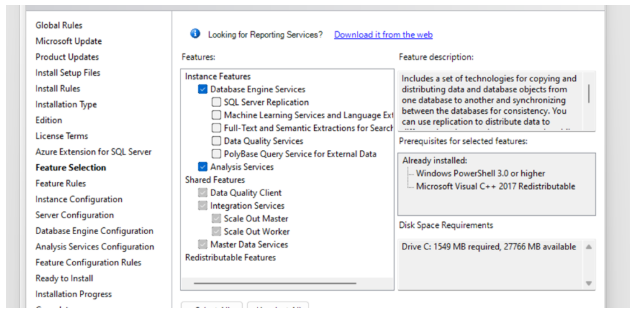
\includegraphics[width=0.5\linewidth]{img/48.png}
\end{figure}
\quad \textbf{Feature selection: SERVER thứ 2 trở con \textrightarrow{} server con chỉ tích như trên. Nếu SERVER đâu tiên server gốc tích hết lựa chọn:}
\begin{figure}[H]
    \centering
    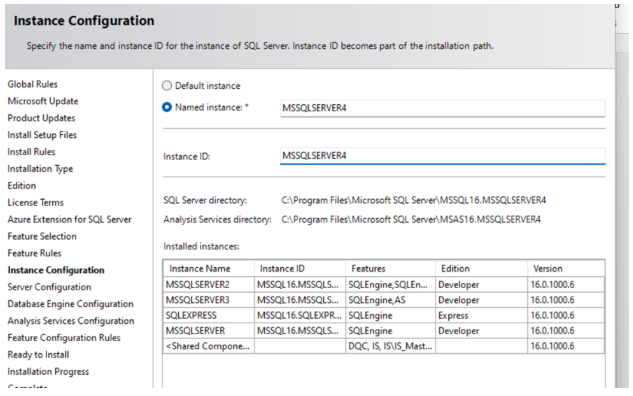
\includegraphics[width=0.5\linewidth]{img/49.png}
\end{figure}
\quad \textbf{Đặt Tên cho server}\
\begin{figure}[H]
    \centering
    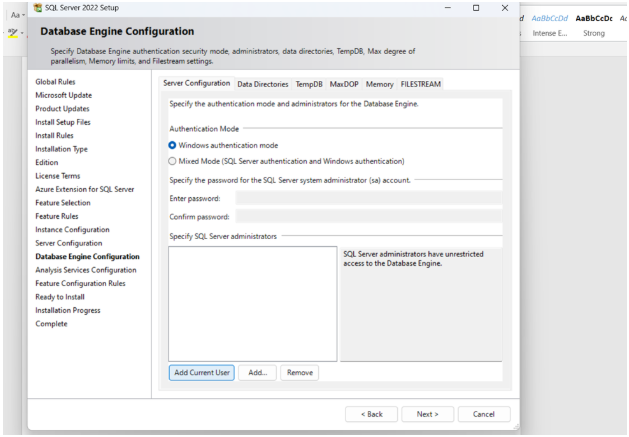
\includegraphics[width=0.5\linewidth]{img/50.png}
\end{figure}
\quad \textbf{Database Engine Configuration:} Chọn mixed Mode (SQL server) \newline
\quad Đặt password dễ \newline
\quad + Cho 3 server nên trùng nhau
\begin{figure}[H]
    \centering
    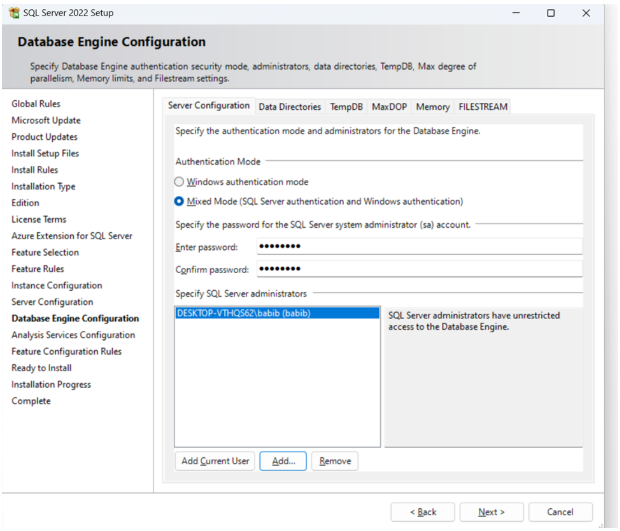
\includegraphics[width=0.5\linewidth]{img/51.png}
\end{figure}
\quad Sau khi đặt password xong, chọn Add Current User: \newline
\quad + Để thêm mới user \newline
\quad + Chọn tiếp Add để thêm Admin \newline
\begin{figure}[H]
    \centering
    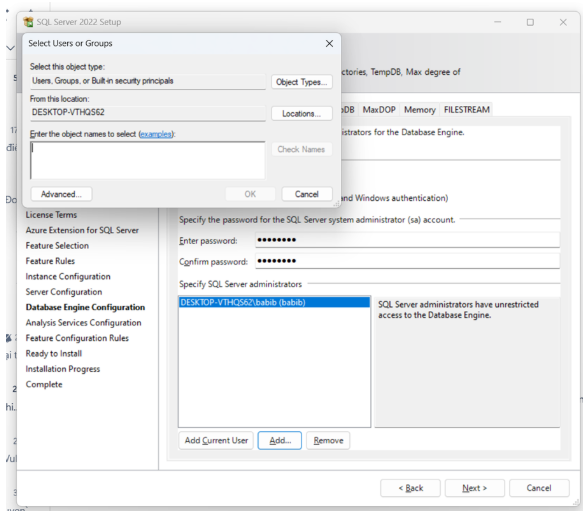
\includegraphics[width=0.5\linewidth]{img/52.png}
\end{figure}
\quad + Chọn Advance \newline
\quad + Chọn Find Now để thêm
\begin{figure}[H]
    \centering
    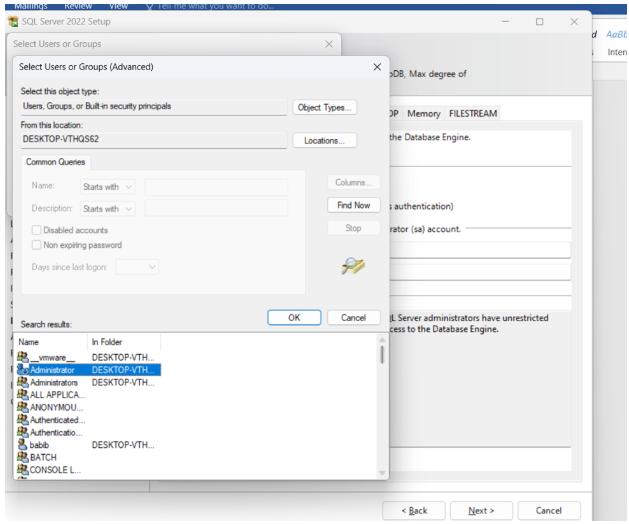
\includegraphics[width=0.5\linewidth]{img/53.png} \hfill
    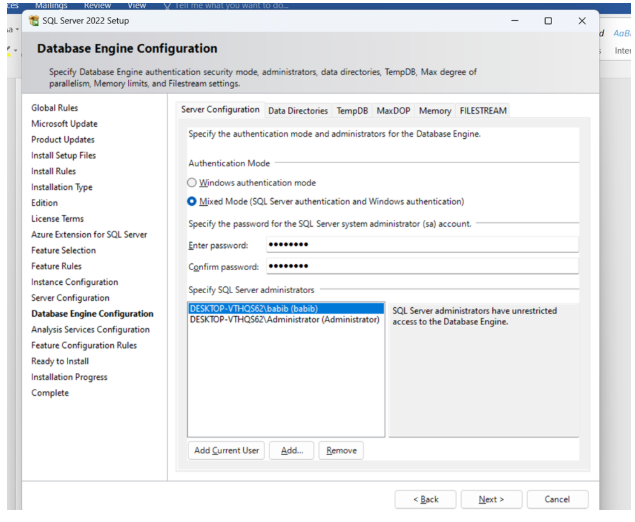
\includegraphics[width=0.5\linewidth]{img/54.png} \\
\end{figure}
\begin{figure}[H]
    \centering
    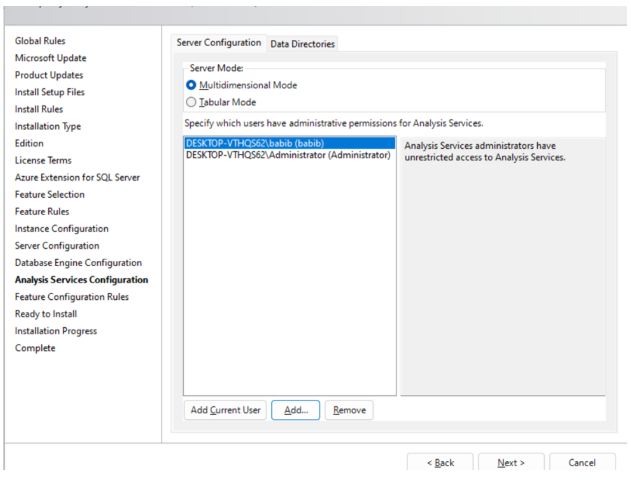
\includegraphics[width=0.5\linewidth]{img/55.png} \hfill 
    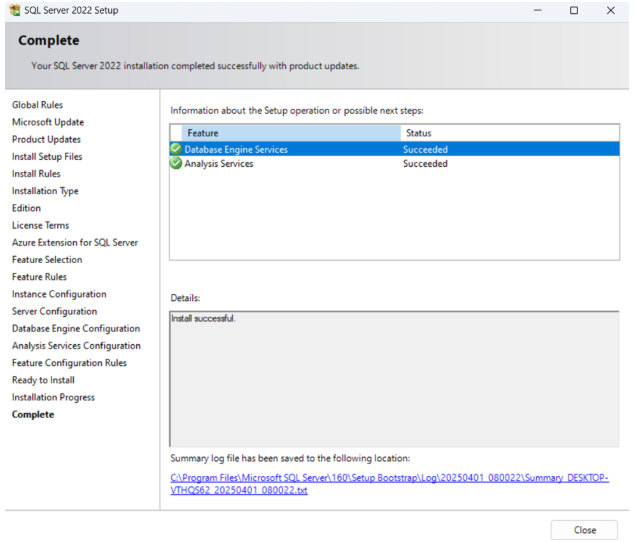
\includegraphics[width=0.5\linewidth]{img/56.png}
\end{figure}
\quad Xong cài đặt
\begin{figure}[H]
    \centering
    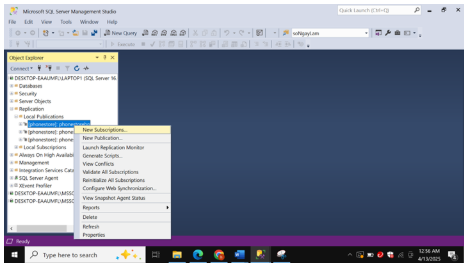
\includegraphics[width=0.5\linewidth]{img/57.png} \hfill
    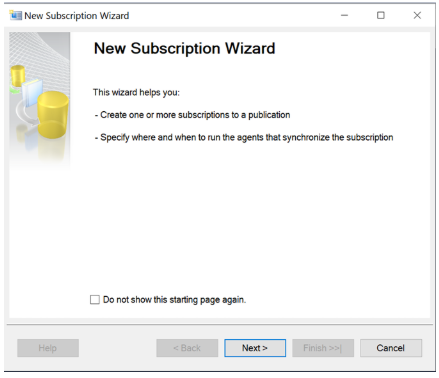
\includegraphics[width=0.5\linewidth]{img/58.png} \\
    \vspace{2mm}
    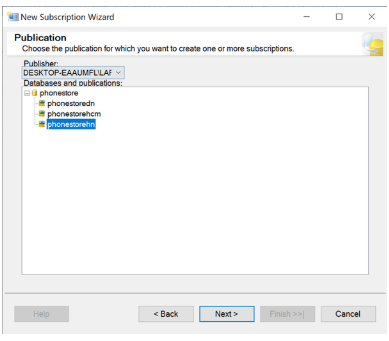
\includegraphics[width=0.45\linewidth]{img/59.png}\hfill
    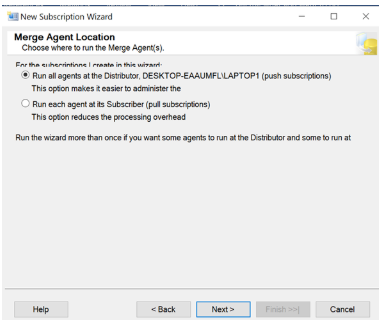
\includegraphics[width=0.45\linewidth]{img/60.png}\\
    \vspace{2mm}
    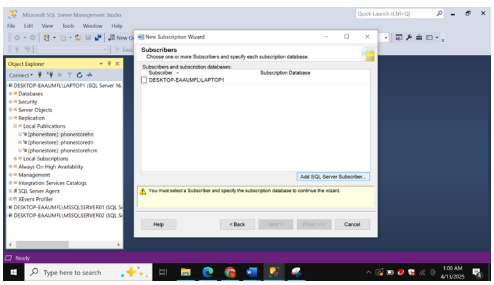
\includegraphics[width=0.5\linewidth]{img/61.png} \hfill
    \caption{ \centering Chọn Subscriber (server sẽ chứa dữ liệu phân tán publication phonestorehn)
    Có thể chọn server khác để chứa dữ liệu phân tán này.
    Add SQL server Subscriber\dots}
\end{figure}
\begin{figure}[H]
    \centering
    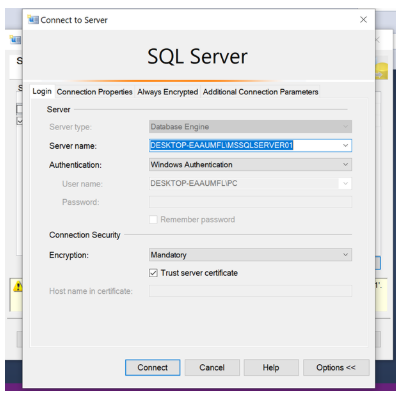
\includegraphics[width=0.45\linewidth]{img/62.png} \hfill
    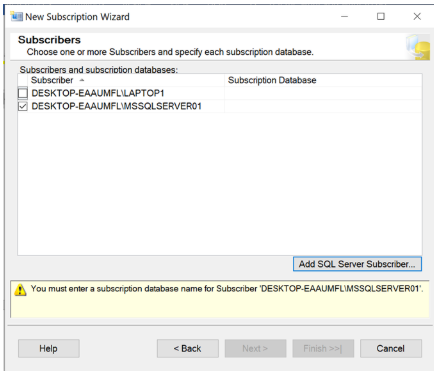
\includegraphics[width=0.45\linewidth]{img/63.png} \\
    \vspace{2mm}
    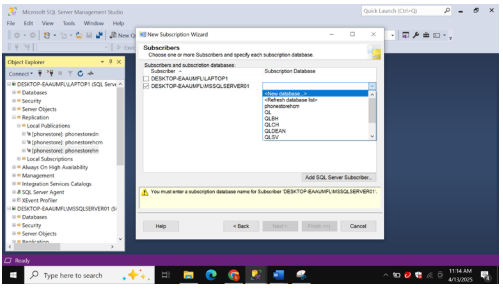
\includegraphics[width=0.45\linewidth]{img/64.png}\hfill
    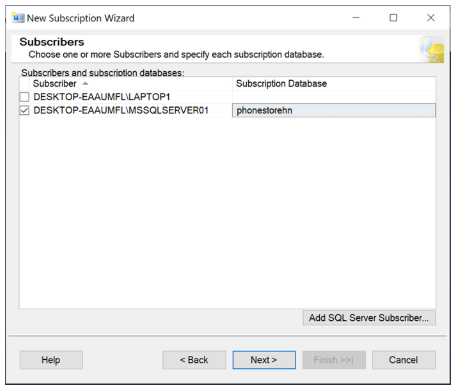
\includegraphics[width=0.45\linewidth]{img/65.png}\\
    \vspace{2mm}
    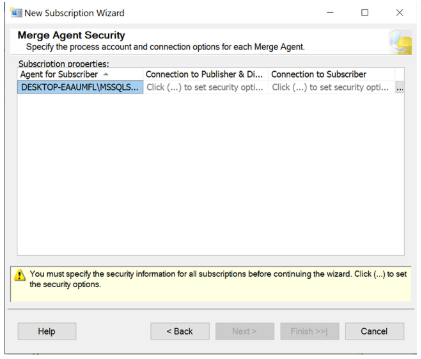
\includegraphics[width=0.45\linewidth]{img/66.png} \hfill
    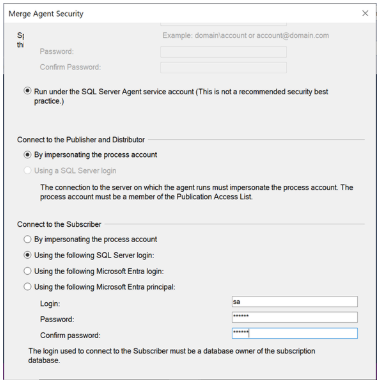
\includegraphics[width=0.45\linewidth]{img/67.png}
    \caption{Tài khoản login vào \textbf{Subscriber (MSSQLSERVER01)}}
\end{figure}
\begin{figure}[H]
    \centering
    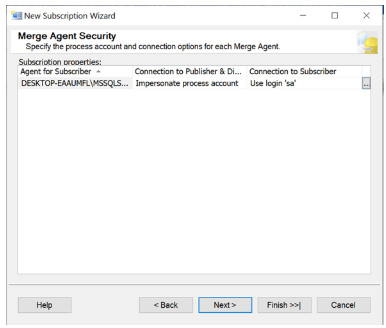
\includegraphics[width=0.5\linewidth]{img/68.png} \hfill
    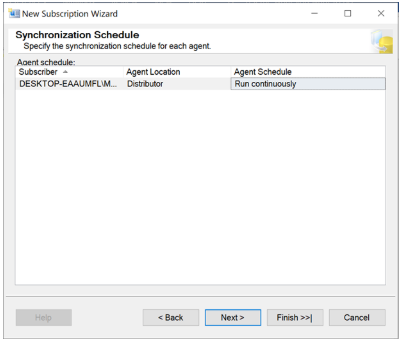
\includegraphics[width=0.5\linewidth]{img/69.png}\\
    \caption{Chọn Run continuously}
\end{figure}
\begin{figure}[H]
    \centering
    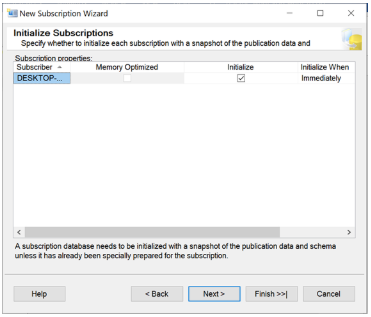
\includegraphics[width=0.45\linewidth]{img/70.png} \hfill
    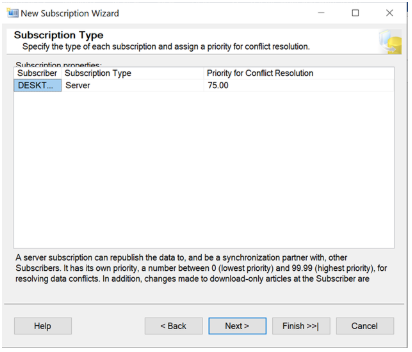
\includegraphics[width=0.45\linewidth]{img/71.png} \\
    \vspace{2mm}
    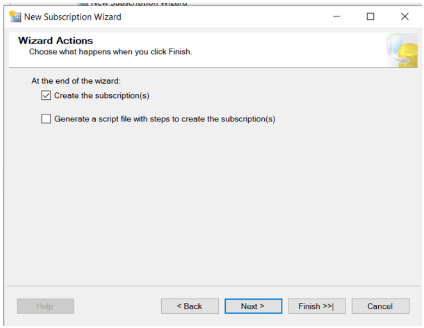
\includegraphics[width=0.45\linewidth]{img/72.png}\hfill
    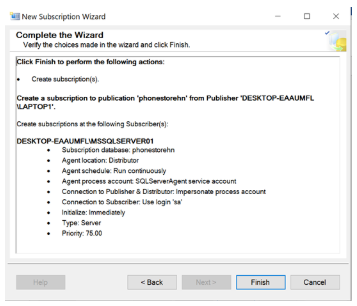
\includegraphics[width=0.45\linewidth]{img/73.png}\\
    \vspace{2mm}
    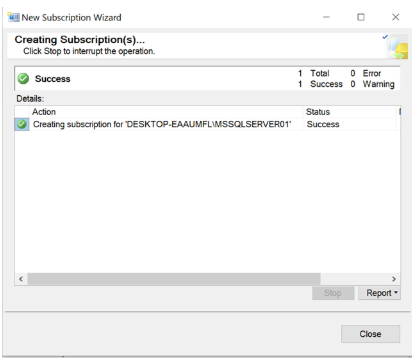
\includegraphics[width=0.45\linewidth]{img/74.png} \hfill
    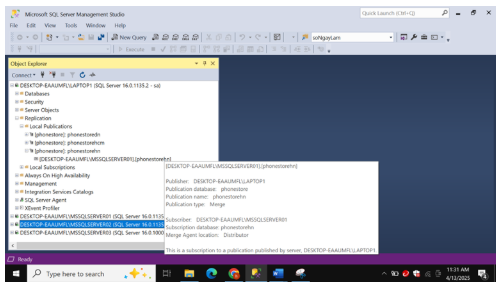
\includegraphics[width=0.45\linewidth]{img/75.png}
\end{figure}
\begin{figure}[H]
    \centering
    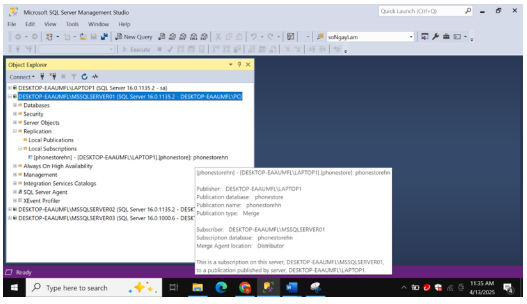
\includegraphics[width=0.45\linewidth]{img/76.png} \\
    \caption{\centering Và database phonestorehn sẽ có các table ứng với các phân mảnh trong publication phonestore}
\end{figure}
\begin{figure}[H]
    \centering
    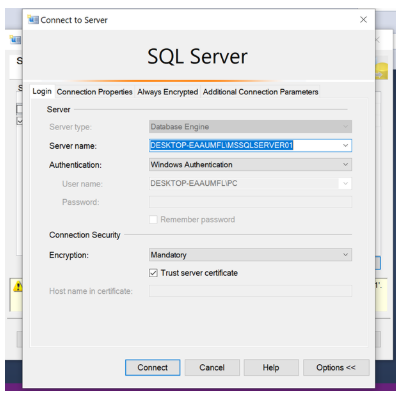
\includegraphics[width=0.45\linewidth]{img/62.png} \hfill
    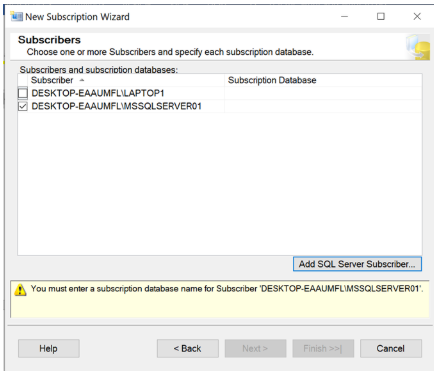
\includegraphics[width=0.45\linewidth]{img/63.png} \\
    \vspace{2mm}
    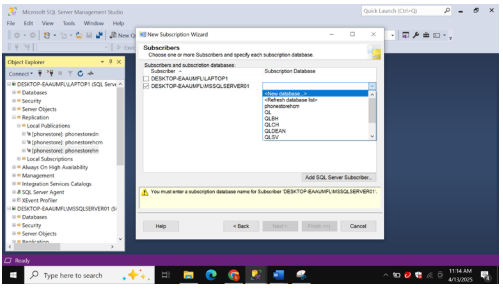
\includegraphics[width=0.45\linewidth]{img/64.png}\hfill
    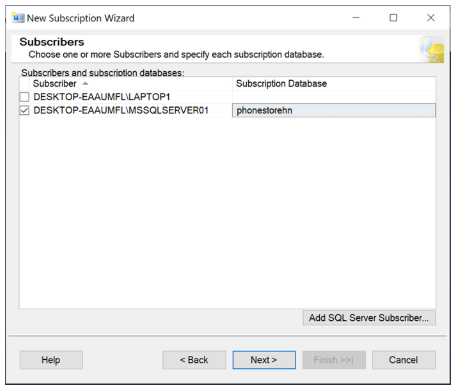
\includegraphics[width=0.45\linewidth]{img/65.png}\\
    \vspace{2mm}
    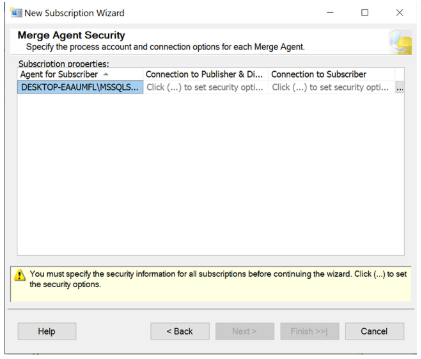
\includegraphics[width=0.45\linewidth]{img/66.png} \hfill
    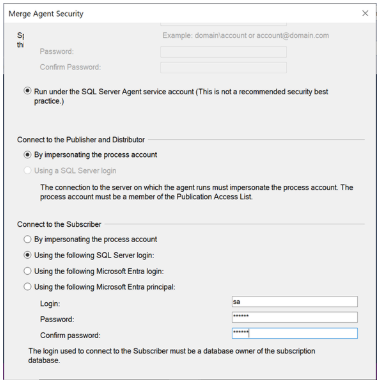
\includegraphics[width=0.45\linewidth]{img/67.png}
    \caption{Tài khoản login vào \textbf{Subscriber (MSSQLSERVER01)}}
\end{figure}
\subsection{Cài đặt Linked Server}
\begin{itemize}[label=*]
    \item Để connect giữa các server này ta có thể tạo link server
    \begin{figure}[H]
        \centering
        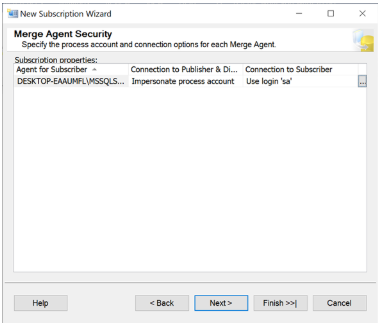
\includegraphics[width=0.5\linewidth]{img/78.png}
    \end{figure}
\end{itemize}
\begin{itemize}
    \item Quy tắc:
          \begin{itemize}
              \item Tên các csdl ở các server subscriber phải giống nhau
              \item Tên link server phải giống nhau
          \end{itemize}
    \item Các bước thực hiện sau:
          \begin{enumerate}[label=Bước \arabic*:]
              \item Tạo remotelogin tên "HTKN" (Hỗ trợ kết nối - dùng cho phép connect) ở cả 4 server
              \item Phân quyền account "HTKN" cho thấy database "phonestore"
              \item Tạo linked server như sau:
                    \begin{itemize}[label=+]
                        \item Trên server gốc tạo linked server LINK1, LINK2, LINK3 lần~lượt trỏ đến server 1, server 2, server 3
                        \item Trên server 1 tạo linked server LINK0, LINK2, LINK3 lần lượt trỏ đến server gốc, server 2, server 3
                        \item Trên server 2 tạo linked server LINK0, LINK1, LINK3 lần lượt trỏ đến server gốc, server 1, server 3
                        \item Trên server 3 tạo linked server LINK0, LINK1, LINK2 lần lượt trỏ đến server gốc, server 1, server 2
                    \end{itemize}

                    \begin{figure}[H]
                        \centering
                        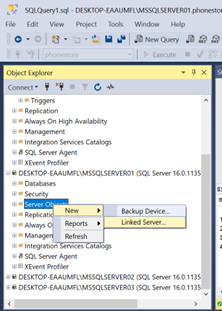
\includegraphics[width=0.4\linewidth]{../HTTDN/image/Bao-cao-HTTTDN/43.png} \hfill
                        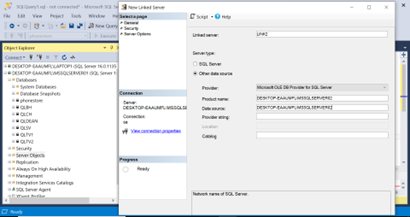
\includegraphics[width=0.45\linewidth]{../HTTDN/image/Bao-cao-HTTTDN/44.png} \\
                        \vspace{2mm}
                        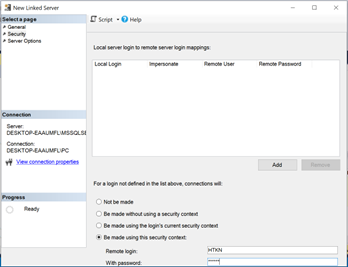
\includegraphics[width=0.45\linewidth]{../HTTDN/image/Bao-cao-HTTTDN/45.png} \hfill
                        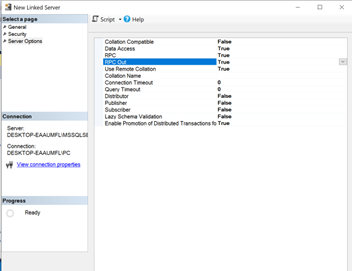
\includegraphics[width=0.45\linewidth]{../HTTDN/image/Bao-cao-HTTTDN/46.png} \\
                    \end{figure}

                    \begin{itemize}
                        \item RPC (Remote Procedure Call): Cho phép máy chủ SQL hiện tại có thể chạy thủ tục lưu trữ (Stored Procedures) từ linked server (máy chủ liên kết). Tức là bạn có thể gọi thủ tục từ server khác như: \newline \texttt{EXEC [LinkedServerName].DatabaseName.dbo.StoredProcedureName}
                        \item RPC Out: Cho phép linked server gọi Stored Procedures trên chính máy chủ hiện tại
                        \item Nghĩa là nếu máy chủ A liên kết đến B và RPC Out = True, thì B có thể gọi thủ tục trên A.
                    \end{itemize}

                    \textbf{Chú ý:} Tạo linked server LINK0 tại server gốc để tránh bị báo lỗi khi truy vấn \newline
                    \begin{figure}[H]
                        \centering
                        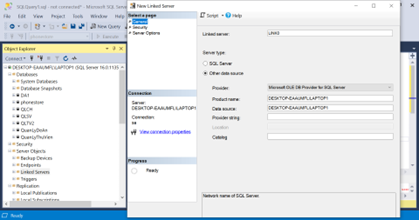
\includegraphics[width=0.5\linewidth]{../HTTDN/image/Bao-cao-HTTTDN/47.png} \\
                        \vspace{2mm}
                        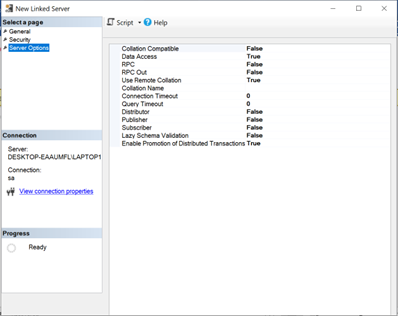
\includegraphics[width=0.5\linewidth]{../HTTDN/image/Bao-cao-HTTTDN/48.png}
                    \end{figure}
          \end{enumerate}
\end{itemize}


\section{Các truy vấn và thao tác với cơ sở dữ liệu phân tán}
\subsection{Các truy dữ liệu ở Server gốc}
\subsubsection{Chức năng quản lý nhân viên}
\begin{itemize}[label=\textbf{-}]
    \item \textbf{Lấy danh sách nhân viên tất cả các kho} \newline
    \begin{lstlisting}[language=SQL, basicstyle=\ttfamily\small]
CREATE PROCEDURE sp_LayDanhSachNhanVienGoc
AS
BEGIN
    SET NOCOUNT ON;
    SELECT * FROM LINK1.phonestore.dbo.NHANVIEN 
    WHERE trangThai = 'on'
    UNION ALL

    SELECT * FROM LINK2.phonestore.dbo.NHANVIEN 
    WHERE trangThai = 'on'
    UNION ALL

    SELECT * FROM LINK3.phonestore.dbo.NHANVIEN 
    WHERE trangThai = 'on'
END
\end{lstlisting}
    Kết quả truy vấn
    \begin{figure}[H]
        \centering
        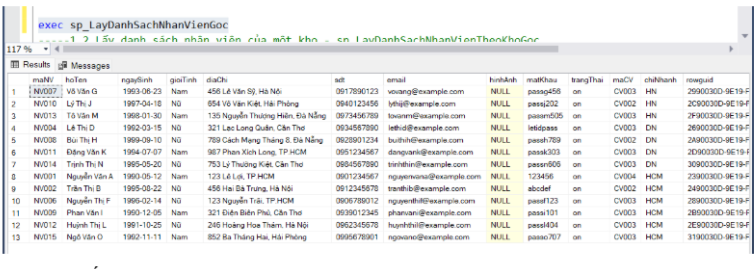
\includegraphics[width=0.8\linewidth]{img/1-1.png}
    \end{figure}
    \item \textbf{Lấy danh sách nhân viên của một kho} \newline
\begin{lstlisting}[language=SQL, basicstyle=\ttfamily\small]
    CREATE PROCEDURE sp_LayDanhSachNhanVienTheoKhoGoc
    @maKho VARCHAR(10)
AS
BEGIN
    SET NOCOUNT ON;
    IF @maKho = 'HN'
    BEGIN
        SELECT *, 'HN' AS chiNhanh 
        FROM LINK1.[phonestore].dbo.NHANVIEN 
        WHERE trangThai = 'on'
    END
    ELSE IF @maKho = 'DN'
    BEGIN
        SELECT *, 'DN' AS chiNhanh 
        FROM LINK2.[phonestore].dbo.NHANVIEN 
        WHERE trangThai = 'on'
    END
    ELSE IF @maKho = 'HCM'
    BEGIN
        SELECT *, 'HCM' AS chiNhanh 
        FROM LINK3.[phonestore].dbo.NHANVIEN 
        WHERE trangThai = 'on'
    END
    ELSE
    BEGIN
        RAISERROR(N'Ma kho khong hop le.', 16, 1)
    END
END

\end{lstlisting}
    Kết quả truy vấn
    \begin{figure}[H]
        \centering
        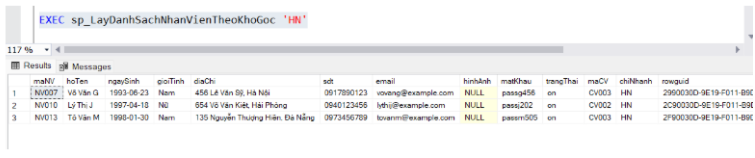
\includegraphics[width=0.8\linewidth]{img/1-2.png}
    \end{figure}
    \item \textbf{Tạo mã nhân viên tự động tăng} \newline
    \begin{lstlisting}[language=SQL, basicstyle=\ttfamily\small]
        create procedure sp_TaoMaNhanVien
        @mamoi varchar(10) OUTPUT
as
begin
    declare @sl1 INT = 0
    declare @sl2 INT = 0
    declare @sl3 INT = 0
    declare @tongSoLuong INT, @soThuTu INT
    select @sl1 = COUNT(*) 
    FROM LINK1.PHONESTORE.dbo.NHANVIEN
    select @sl2 = COUNT(*) 
    FROM LINK2.PHONESTORE.dbo.NHANVIEN
    select @sl3 = COUNT(*) 
    FROM LINK3.PHONESTORE.dbo.NHANVIEN
    set @tongSoLuong = @sl1 + @sl2 + @sl3
    SET @soThuTu = @tongSoLuong + 1
    set @mamoi = 'NV' + RIGHT('000'+CONVERT(VARCHAR, @soThuTu), 3)
END
        
        \end{lstlisting}
        \begin{figure}[H]
            \centering
            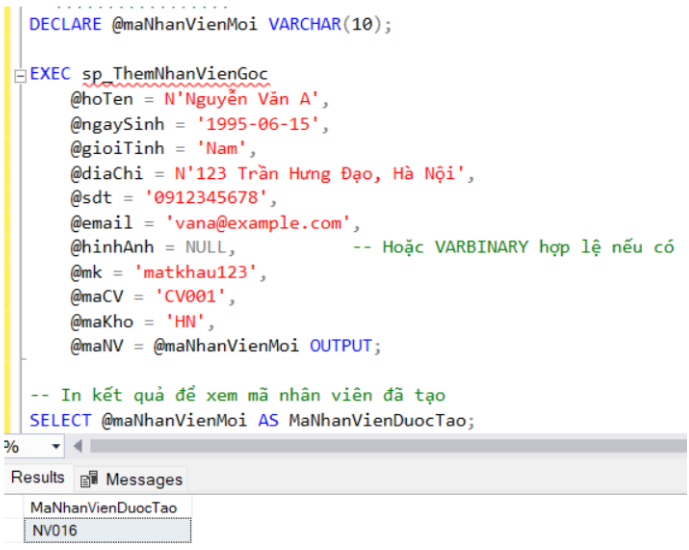
\includegraphics[width=0.8\linewidth]{img/1-3.png}
        \end{figure}
    \item \textbf{Thêm nhân viên} \newline
    \begin{lstlisting}[language=SQL, basicstyle=\ttfamily\small]
        CREATE PROCEDURE sp_ThemNhanVienGoc
        @hoTen NVARCHAR(100),
        @ngaySinh DATE,
        @gioiTinh NVARCHAR(3),
        @diaChi NVARCHAR(200),
        @sdt NVARCHAR(20),
        @email NVARCHAR(255),
        @hinhAnh VARBINARY(MAX),
        @matKhau NVARCHAR(200),
        @maCV NVARCHAR(50),
        @maKho VARCHAR(10)
AS
BEGIN
    SET NOCOUNT ON;
    DECLARE @maNV VARCHAR(10)
-- 1. Tao ma nha vien moi duy nhat
    EXEC sp_TaoMaNhanVien @maNV OUTPUT
-- 2. Goi toi dung thu tuc o server phan manh de them nhan vien cuc bo
    IF @maKho = 'HN'
    BEGIN
        EXEC LINK1.phonestore.dbo.sp_ThemNhanVienKho
        @hoTen, @ngaySinh, @gioiTinh, @diaChi, @sdt, @email,
        @hinhAnh, @matKhau, @maCV, @maKho, @maNV OUTPUT
    END
    ELSE IF @maKho = 'DN'
    BEGIN
        EXEC LINK2.phonestore.dbo.sp_ThemNhanVienKho
            @hoTen, @ngaySinh, @gioiTinh, @diaChi, @sdt, @email,
            @hinhAnh, @matKhau, @maCV, @maKho, @maNV OUTPUT
    END
    ELSE IF @maKho = 'HCM'
    BEGIN
        EXEC LINK3.phonestore.dbo.sp_ThemNhanVienKho
            @hoTen, @ngaySinh, @gioiTinh, @diaChi, @sdt, @email,
            @hinhAnh, @matKhau, @maCV, @maKho, @maNV OUTPUT
    END
    ELSE
    BEGIN
        RAISERROR(N'Ma kho khong hop le.', 16, 1)
        RETURN
    END
END
        \end{lstlisting}
    Kết quả truy vấn
    \begin{figure}[H]
        \centering
        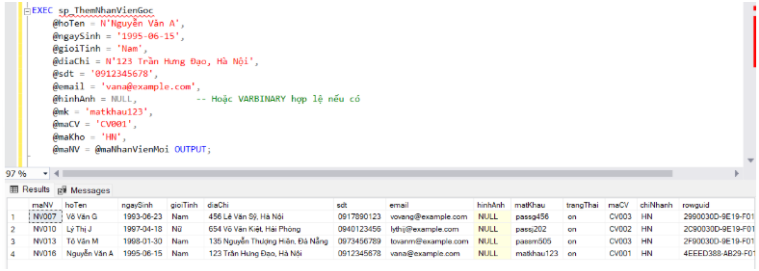
\includegraphics[width=0.8\linewidth]{img/1-4.png}
    \end{figure}
    \item \textbf{Tìm nhân viên theo manv} \newline
    \begin{lstlisting}[language=SQL, basicstyle=\ttfamily\small]
        CREATE PROCEDURE sp_TimNhanVienTheoMaNVGoc
        @maNV VARCHAR(10)
AS
BEGIN
    SET NOCOUNT ON;
-- Tim o phan manh HN
    IF EXISTS (SELECT 1 FROM LINK1.phonestore.dbo.NHANVIEN 
    WHERE maNV = @maNV)
    BEGIN
        SELECT *, N'HN' AS chiNhanh 
        FROM LINK1.phonestore.dbo.NHANVIEN
        WHERE maNV = @maNV;
        RETURN;
        END
-- Tim o phan manh DN
    IF EXISTS (SELECT 1 FROM LINK2.phonestore.dbo.NHANVIEN 
    WHERE maNV = @maNV)
    BEGIN
        SELECT *, N'DN' AS chiNhanh 
        FROM LINK2.phonestore.dbo.NHANVIEN
        WHERE maNV = @maNV;
        RETURN;
    END
-- Tim o phan manh HCM
    IF EXISTS (SELECT 1 FROM LINK3.phonestore.dbo.NHANVIEN 
    WHERE maNV = @maNV)
    BEGIN
        SELECT *, N'HCM' AS chiNhanh 
        FROM LINK3.phonestore.dbo.NHANVIEN
        WHERE maNV = @maNV;
        RETURN;
    END
    RAISERROR(N'Khong tim thay nhan vien voi ma da cho.', 16, 1);
END
    
        \end{lstlisting}
        Kết quả truy vấn
        \begin{figure}[H]
            \centering
            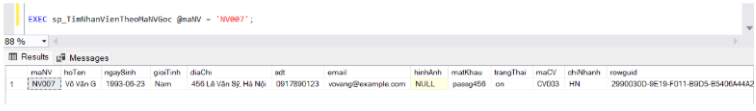
\includegraphics[width=0.8\linewidth]{img/1-5.png}
        \end{figure}
\end{itemize}
\subsubsection{Chức năng quản lý bảng chấm công}
\begin{itemize}[label=\textbf{-}]
    \item \textbf{Lấy danh sách bảng chấm công} \newline
    \begin{lstlisting}[language=SQL, basicstyle=\ttfamily\small]
drop procedure sp_LayDSChamCongGoc
CREATE PROCEDURE sp_LayDSChamCongGoc
AS
BEGIN
    SET NOCOUNT ON;
    SELECT * FROM LINK1.phonestore.dbo.BANGCHAMCONG
    UNION ALL
    SELECT * FROM LINK2.phonestore.dbo.BANGCHAMCONG
    UNION ALL
    SELECT * FROM LINK3.phonestore.dbo.BANGCHAMCONG
END
\end{lstlisting}
    Kết quả truy vấn
    \begin{figure}[H]
        \centering
        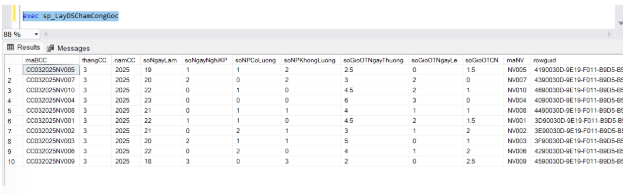
\includegraphics[width=0.8\linewidth]{img/79.png}
    \end{figure}
    \item \textbf{Lấy danh sách bảng chấm công của một kho} \newline
\begin{lstlisting}[language=SQL, basicstyle=\ttfamily\small]
    create procedure sp_DSBangChamCongTheoKhoGoc
    @maKho VARCHAR(10) -- Ma kho can lay danh sach cham cong
AS
BEGIN
    SET NOCOUNT ON;
    DECLARE @ServerLink NVARCHAR(100)
    -- Gan server tuong ung voi ma kho
    IF @maKho = 'HN' SET @ServerLink = 'LINK1'
    ELSE IF @maKho = 'DN' SET @ServerLink = 'LINK2'
    ELSE IF @maKho = 'HCM' SET @ServerLink = 'LINK3'
    ELSE
    BEGIN
        RAISERROR('Kho khong hop le', 16, 1)
        RETURN
    END

    -- Truy van danh sach cham cong tu kho tuong ung
    DECLARE @SQL NVARCHAR(MAX)
    SET @SQL = '
        SELECT *
        FROM [' + @ServerLink + '].phonestore.dbo.BANGCHAMCONG
        ORDER BY thangCC DESC, namCC DESC'

    -- Thuc thi cau lanh SQL dong
    EXEC sp_executesql @SQL
END


\end{lstlisting}
    Kết quả truy vấn
    \begin{figure}[H]
        \centering
        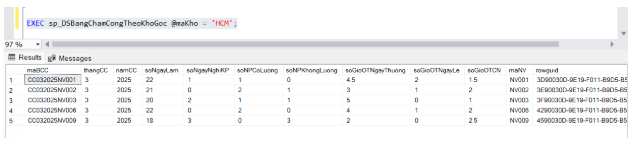
\includegraphics[width=0.8\linewidth]{img/80.png}
    \end{figure}
    \item \textbf{Lấy danh sách bảng chấm công theo thời gian} \newline
    \begin{lstlisting}[language=SQL, basicstyle=\ttfamily\small]
        CREATE PROCEDURE sp_LayDSBangChamCongTheoTGGoc
    @thangCC INT,
    @namCC INT
AS
BEGIN
    SET NOCOUNT ON;

    DECLARE @sql NVARCHAR(MAX);

    SET @sql = '
    SELECT * FROM OPENQUERY(LINK1,
        ''SELECT * FROM phonestore.dbo.BANGCHAMCONG 
          WHERE thangCC = ' + CAST(@thangCC AS NVARCHAR) 
          + ' AND namCC = ' + CAST(@namCC AS NVARCHAR) + ''')
    UNION ALL
    SELECT * FROM OPENQUERY(LINK2,
        ''SELECT * FROM phonestore.dbo.BANGCHAMCONG 
          WHERE thangCC = ' + CAST(@thangCC AS NVARCHAR) 
          + ' AND namCC = ' + CAST(@namCC AS NVARCHAR) + ''')
    UNION ALL
    SELECT * FROM OPENQUERY(LINK3,
        ''SELECT * FROM phonestore.dbo.BANGCHAMCONG 
          WHERE thangCC = ' + CAST(@thangCC AS NVARCHAR) 
          + ' AND namCC = ' + CAST(@namCC AS NVARCHAR) + ''')';
    EXEC sp_executesql @sql;
END

        \end{lstlisting}
        \begin{figure}[H]
            \centering
            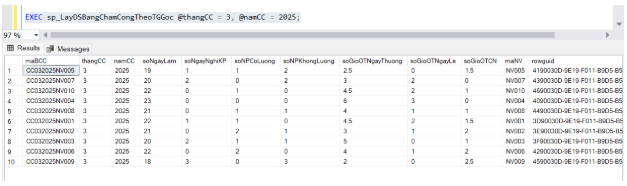
\includegraphics[width=0.8\linewidth]{img/81.png}
        \end{figure}
    \item \textbf{Thêm bảng chấm công} \newline
    \begin{lstlisting}[language=SQL, basicstyle=\ttfamily\small]
        CREATE PROCEDURE sp_ThemChamCongGoc
    @maCC VARCHAR(50),
    @thangCC INT,
    @namCC INT,
    @soNgayLam FLOAT = NULL,
    @soNgayNghiKP FLOAT = NULL,
    @soNPCoLuong FLOAT = NULL,
    @soNPKhongLuong FLOAT = NULL,
    @soGioOTNgayThuong FLOAT = NULL,
    @soGioOTNgayLe FLOAT = NULL,
    @soGioOTCN FLOAT = NULL,
    @maNV VARCHAR(50)
AS
BEGIN
    SET NOCOUNT ON;

    DECLARE @found BIT = 0;

    -- Kiem tra LINK1
    IF EXISTS (
        SELECT 1
        FROM LINK1.phonestore.dbo.NHANVIEN
        WHERE maNV = @maNV
    )
    BEGIN
        EXEC LINK1.phonestore.dbo.sp_ThemChamCongKho
            @maCC, @thangCC, @namCC,
            @soNgayLam, @soNgayNghiKP, @soNPCoLuong,
            @soNPKhongLuong,@soGioOTNgayThuong, 
            @soGioOTNgayLe, @soGioOTCN, @maNV;
        SET @found = 1;
        RETURN;
    END

    -- Kiem tra LINK2
    IF EXISTS (
        SELECT 1
        FROM LINK2.phonestore.dbo.NHANVIEN
        WHERE maNV = @maNV
    )
    BEGIN
        EXEC LINK2.phonestore.dbo.sp_ThemChamCongKho
            @maCC, @thangCC, @namCC,
            @soNgayLam, @soNgayNghiKP, @soNPCoLuong, 
            @soNPKhongLuong, @soGioOTNgayThuong, 
            @soGioOTNgayLe, @soGioOTCN, @maNV;
        SET @found = 1;
        RETURN;
    END

    -- Kiem tra LINK3
    IF EXISTS (
        SELECT 1
        FROM LINK3.phonestore.dbo.NHANVIEN
        WHERE maNV = @maNV
    )
    BEGIN
        EXEC LINK3.phonestore.dbo.sp_ThemChamCongKho
            @maCC, @thangCC, @namCC,
            @soNgayLam, @soNgayNghiKP, @soNPCoLuong, 
            @soNPKhongLuong, @soGioOTNgayThuong, 
            @soGioOTNgayLe, @soGioOTCN, @maNV;
        SET @found = 1;
        RETURN;
    END

    -- Khong tim thay ma nhan vien
    IF @found = 0
    BEGIN
        RAISERROR(N'Khong tim thay nhan vien trong he thong. 
        Khong the them cham cong.', 16, 1);
    END
END

        \end{lstlisting}
    Kết quả truy vấn
    \begin{figure}[H]
        \centering
        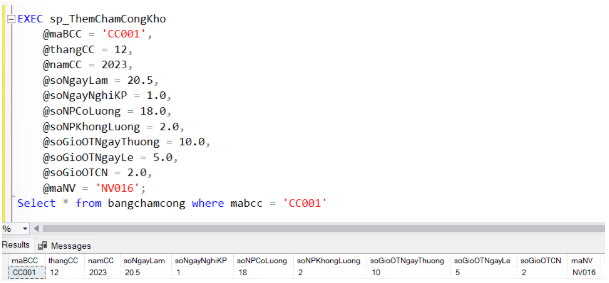
\includegraphics[width=0.8\linewidth]{img/82.png}
    \end{figure}
    \item \textbf{Sửa bảng chấm công} \newline
    \begin{lstlisting}[language=SQL, basicstyle=\ttfamily\small]
        CREATE PROCEDURE sp_SuaChamCongGoc
        @maCC VARCHAR(50),
        @thangCC INT,
        @namCC INT,
        @soNgayLam FLOAT = NULL,
        @soNgayNghiKP FLOAT = NULL,
        @soNPCoLuong FLOAT = NULL,
        @soNPKhongLuong FLOAT = NULL,
        @soGioOTNgayThuong FLOAT = NULL,
        @soGioOTNgayLe FLOAT = NULL,
        @soGioOTCN FLOAT = NULL,
        @maNV VARCHAR(50)
AS
BEGIN
    SET NOCOUNT ON;
    
    DECLARE @found BIT = 0;
    
    -- Phan manh 1: LINK1
    IF EXISTS (
        SELECT 1 FROM LINK1.phonestore.dbo.BANGCHAMCONG
        WHERE maBCC = @maCC)
    BEGIN
        EXEC LINK1.phonestore.dbo.sp_SuaChamCongKho
            @maCC, @thangCC, @namCC,
            @soNgayLam, @soNgayNghiKP, @soNPCoLuong, 
            @soNPKhongLuong, @soGioOTNgayThuong, 
            @soGioOTNgayLe, @soGioOTCN, @maNV;
            SET @found = 1;
            RETURN;
        END
        -- Phan manh 2: LINK2
    IF EXISTS (
        SELECT 1 FROM LINK2.phonestore.dbo.BANGCHAMCONG
        WHERE maBCC = @maCC)
    BEGIN
        EXEC LINK2.phonestore.dbo.sp_SuaChamCongKho
            @maCC, @thangCC, @namCC,
            @soNgayLam, @soNgayNghiKP, @soNPCoLuong, 
            @soNPKhongLuong, @soGioOTNgayThuong, 
            @soGioOTNgayLe, @soGioOTCN, @maNV;
            SET @found = 1;
            RETURN;
        END
    
        -- Phan manh 3: LINK3
    IF EXISTS (
        SELECT 1 FROM LINK3.phonestore.dbo.BANGCHAMCONG
            WHERE maBCC = @maCC)
    BEGIN
        EXEC LINK3.phonestore.dbo.sp_SuaChamCongKho
            @maCC, @thangCC, @namCC,
            @soNgayLam, @soNgayNghiKP, @soNPCoLuong, 
            @soNPKhongLuong, @soGioOTNgayThuong, 
            @soGioOTNgayLe, @soGioOTCN, @maNV;
        SET @found = 1;
            RETURN;
    END
    
        -- Khong tim thay ma cham cong
    IF @found = 0
    BEGIN
        RAISERROR(N'Ma cham cong khong ton tai trong toan he thong.', 16, 1);
    END
END
        \end{lstlisting}
        Kết quả truy vấn
        \begin{figure}[H]
            \centering
            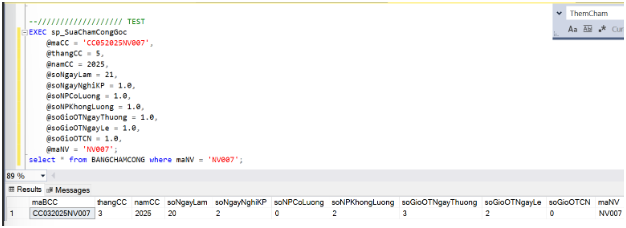
\includegraphics[width=0.8\linewidth]{img/83.png}
        \end{figure}
    \item \textbf{Tìm bảng chấm công theo maBCC} \newline
        \begin{lstlisting}[language=SQL, basicstyle=\ttfamily\small]
            CREATE PROCEDURE sp_TimBangCCTheoMaBCCGoc 
            @maBCC VARCHAR(50)
AS
BEGIN
    SET NOCOUNT ON;
    DECLARE @found BIT = 0;
    -- Kiem tra tai LINK1
    IF EXISTS (
    SELECT 1 FROM LINK1.phonestore.dbo.BANGCHAMCONG
    WHERE maBCC = @maBCC)
    BEGIN
        EXEC LINK1.phonestore.dbo.sp_TimBangCCTheoMaBCCKho @maBCC;
        SET @found = 1;
        RETURN;
    END
            -- Kiem tra tai LINK2
    IF EXISTS (
    SELECT 1 FROM LINK2.phonestore.dbo.BANGCHAMCONG
    WHERE maBCC = @maBCC)
    BEGIN
        EXEC LINK2.phonestore.dbo.sp_TimBangCCTheoMaBCCKho @maBCC;
        SET @found = 1;
        RETURN;
    END
    -- Kiem tra tai LINK3
    IF EXISTS (
    SELECT 1 FROM LINK3.phonestore.dbo.BANGCHAMCONG
    WHERE maBCC = @maBCC)
    BEGIN
        EXEC LINK3.phonestore.dbo.sp_TimBangCCTheoMaBCCKho @maBCC;
        SET @found = 1;
        RETURN;
    END
    -- Neu khong tim thay
    IF @found = 0
    BEGIN
        RAISERROR(N'Khong tim thay bang cham cang voi ma da nhap 
        trong toan he thong.', 16, 1);
    END
END
            \end{lstlisting}
            Kết quả truy vấn
            \begin{figure}[H]
                \centering
                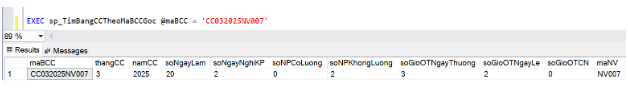
\includegraphics[width=0.8\linewidth]{img/84.png}
            \end{figure}
\end{itemize}
    
\subsection{Các truy vấn dữ liệu ở Server phân mảnh}
Sau khi đã tạo các Stored Procedure ở server gốc, ta tiến hành phân tán chúng xuống cơ sở dữ liệu mảnh \newline
\quad - Ở server gốc, chọn procedure cần phân tán xuống CSDL mảnh
\begin{figure}[H]
    \centering
    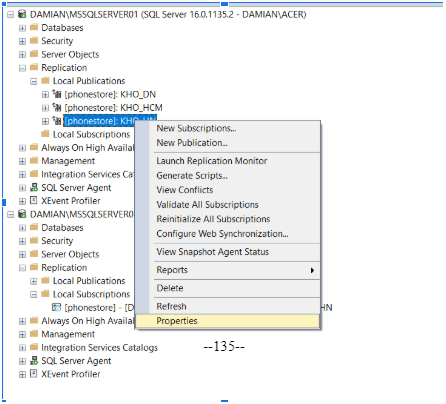
\includegraphics[width=0.5\linewidth]{img/85.png} \hfill
    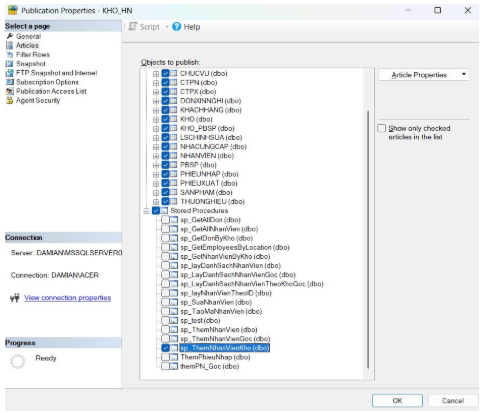
\includegraphics[width=0.5\linewidth]{img/86.png}
\end{figure}
\quad - Nhấn “OK” ư+\newline
\quad - Sau đó chọn "Reinitialize All Subscriptions" đề đồng bộ lại toàn bộ dữ liệu từ đầu (re-sync).
\begin{figure}[H]
    \centering
    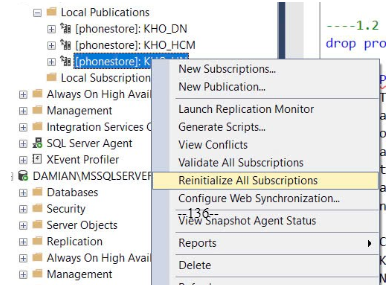
\includegraphics[width=0.5\linewidth]{img/87.png}
\end{figure}
\quad - Sau đó chọn "View Snapshot Agent Status" và chọn Start để đẩy dữ liệu xuống mảnh
\begin{figure}[H]
    \centering
    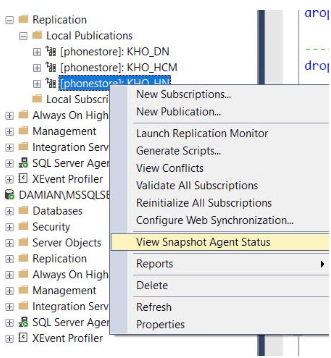
\includegraphics[width=0.5\linewidth]{img/88.png} \hfill
    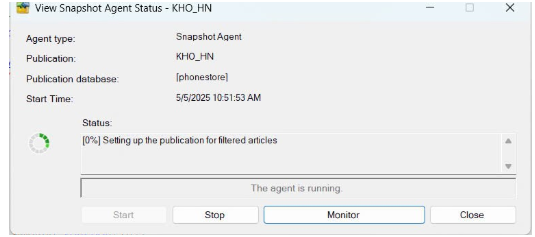
\includegraphics[width=0.5\linewidth]{img/89.png} \\
    \vspace{2mm}
    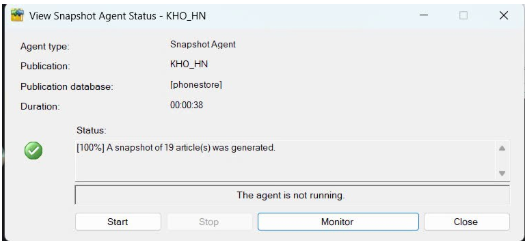
\includegraphics[width=0.5\linewidth]{img/90.png} \hfill
    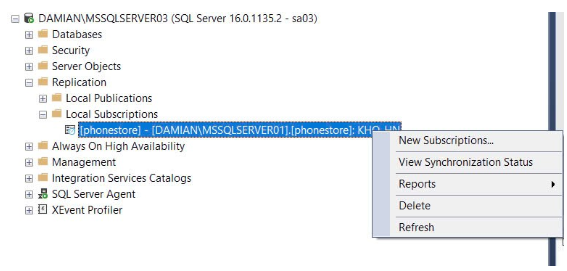
\includegraphics[width=0.5\linewidth]{img/91.png}
\end{figure}
\quad - Ở server mảnh, vào Replication chọn Local Subscriptions và chuột phải vào Subscription, chọn "View Synchronization Status" \newline
\quad - Lúc này hệ thống sẽ yêu cầu kết nối tới server gốc, lúc này ta kết nối 	tới server gốc
\begin{figure}[H]
    \centering
    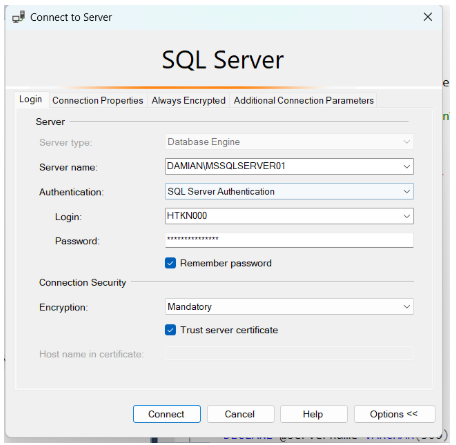
\includegraphics[width=0.5\linewidth]{img/92.png} \hfill
    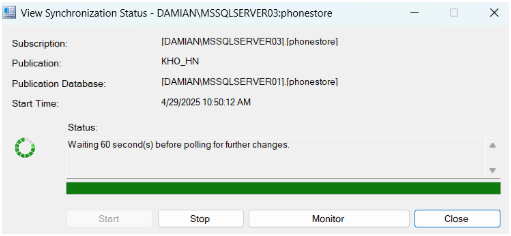
\includegraphics[width=0.5\linewidth]{img/93.png} \\
    \caption{Sau đó chọn Start và chờ đồng bộ dữ liệu}
\end{figure}
\subsubsection{Chức năng quản lý nhân viên}
\textbf{Lấy danh sách nhân viên }
\begin{lstlisting}[language=SQL, basicstyle=\ttfamily\small]
    CREATE PROCEDURE sp_LayDanhSachNhanVienKho
    AS
    BEGIN
        SET NOCOUNT ON;
        SELECT *
        FROM dbo.NHANVIEN;
    END;
\end{lstlisting}
\quad Kết quả truy vấn
\begin{figure}[H]
    \centering
    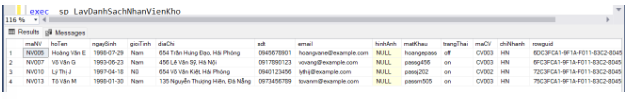
\includegraphics[width=0.8\linewidth]{img/2-1.png}
\end{figure}
\textbf{Thêm nhân viên}
\begin{lstlisting}[language=SQL, basicstyle=\ttfamily\small]
    CREATE PROCEDURE sp_ThemNhanVienKho
    @hoTen NVARCHAR(100),
    @ngaySinh DATE,
    @gioiTinh NVARCHAR(3),
    @diaChi NVARCHAR(200),
    @sdt NVARCHAR(20),
    @email NVARCHAR(255),
    @hinhAnh VARBINARY(MAX),
    @mk NVARCHAR(200),
    @maCV NVARCHAR(50),
    @maKho VARCHAR(10),
    @maNV VARCHAR(10) OUTPUT
AS
BEGIN
    SET NOCOUNT ON;

    DECLARE @servername VARCHAR(300)
    SELECT @servername = @@SERVERNAME

    IF @servername = 'DESKTOP-EAAUMFL\MSSQLSERVER01'
        SET @maKho = 'HN'
    ELSE IF @servername = 'DESKTOP-EAAUMFL\MSSQLSERVER02'
        SET @maKho = 'DN'
    ELSE IF @servername = 'DESKTOP-EAAUMFL\MSSQLSERVER03'
        SET @maKho = 'HCM'

    -- 1. Goi toi server goc de lay ma NV duy nhat
    EXEC LINK0.phonestore.dbo.sp_TaoMaNhanVien @maNV OUTPUT

    -- 2. Kiem tra ma NV da ton tai trong bang cuc bo hay chua
    IF EXISTS (SELECT 1 FROM NHANVIEN WHERE maNV = @maNV)
    BEGIN
        RAISERROR(N'Loi: Ma nhan vien da ton tai trong he thong 
            cuc bo.', 16, 1)
        RETURN
    END

    -- 3. Chen vao bang NHANVIEN cuc bo
    INSERT INTO NHANVIEN
        (maNV, hoTen, ngaySinh, gioiTinh, diaChi, sdt, email, 
        hinhAnh, matKhau, trangThai, maCV, chiNhanh)
    VALUES
        (@maNV, @hoTen, @ngaySinh, @gioiTinh, @diaChi, @sdt, 
        @email, @hinhAnh, @mk, 'on', @maCV, @maKho)
END

\end{lstlisting}
\quad Kết quả truy Xuất
\begin{figure}[H]
    \centering
    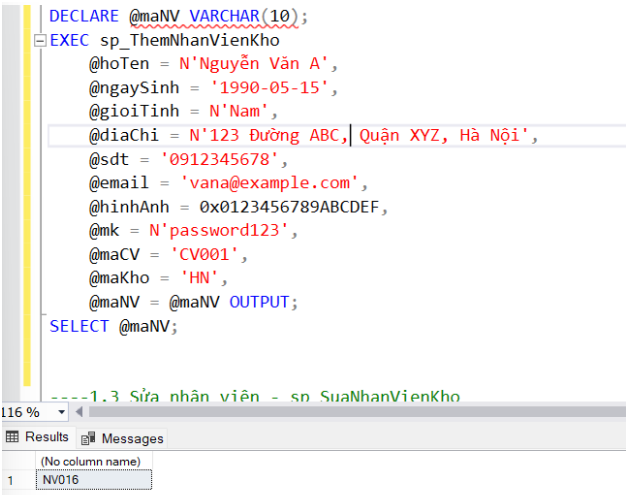
\includegraphics[width=0.8\linewidth]{img/2-2.png}
\end{figure}
\textbf{Sửa nhân viên}
\begin{lstlisting}[language=SQL, basicstyle=\ttfamily\small]
    CREATE PROCEDURE sp_SuaNhanVienKho 
    @maNV VARCHAR(10), 
    @hoTen NVARCHAR(100) = NULL, 
    @ngaySinh DATE = NULL, 
    @gioiTinh NVARCHAR(3) = NULL, 
    @diaChi NVARCHAR(200) = NULL, 
    @sdt NVARCHAR(20) = NULL, 
    @email NVARCHAR(255) = NULL, 
    @hinhAnh VARBINARY(MAX) = NULL, 
    @matKhau NVARCHAR(200) = NULL, 
    @trangThai NVARCHAR(10) = NULL, 
    @maCV NVARCHAR(50) = NULL 
    AS 
    BEGIN 
        SET NOCOUNT ON;
    
        IF EXISTS (SELECT 1 FROM NHANVIEN WHERE maNV = @maNV) 
        BEGIN 
            UPDATE NHANVIEN 
            SET hoTen = ISNULL(@hoTen, hoTen),
                ngaySinh = ISNULL(@ngaySinh, ngaySinh), 
                gioiTinh = ISNULL(@gioiTinh, gioiTinh), 
                diaChi = ISNULL(@diaChi, diaChi), 
                sdt = ISNULL(@sdt, sdt), 
                email = ISNULL(@email, email), 
                hinhAnh = ISNULL(@hinhAnh, hinhAnh), 
                matKhau = ISNULL(@matKhau, matKhau), 
                trangThai = ISNULL(@trangThai, trangThai), 
                maCV = ISNULL(@maCV, maCV) 
            WHERE maNV = @maNV; 
        END 
        ELSE 
        BEGIN 
            RAISERROR(N'Ma nhan vien khong ton tai tai chi 
            nhanh nay.', 16, 1); 
        END 
    END
    \end{lstlisting}
\quad Kết quả truy vấn
\begin{figure}[H]
    \centering
    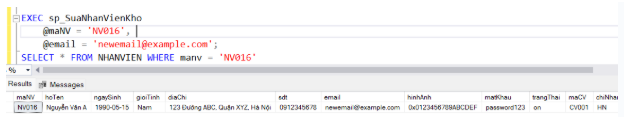
\includegraphics[width=0.8\linewidth]{img/2-3.png}
\end{figure}
\textbf{Tìm kiếm nhân viên theo từ khóa}
\begin{lstlisting}[language=SQL, basicstyle=\ttfamily\small]
    CREATE PROCEDURE sp_TimNhanVienTheoTuKhoaKho
        @tuKhoa NVARCHAR(100)
    AS
    BEGIN
        SET NOCOUNT ON;
    
        SELECT *
        FROM NHANVIEN
        WHERE maNV LIKE '%' + @tuKhoa + '%'
           OR hoTen LIKE '%' + @tuKhoa + '%'
           OR sdt LIKE '%' + @tuKhoa + '%'
           OR email LIKE '%' + @tuKhoa + '%'
    END
    \end{lstlisting}
\quad Kết quả truy vấn
\begin{figure}[H]
    \centering
    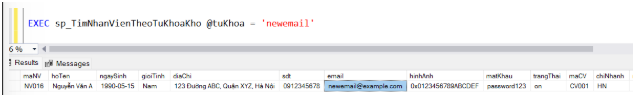
\includegraphics[width=0.8\linewidth]{img/2-4.png}
\end{figure}
\textbf{Tìm kiếm nhân viên theo mã nhân viên}
\begin{lstlisting}[language=SQL, basicstyle=\ttfamily\small]
    CREATE PROCEDURE sp_TimNhanVienTheoMaNVKho
        @maNV VARCHAR(10)
    AS
    BEGIN
        SET NOCOUNT ON;
    
        IF EXISTS (SELECT 1 FROM NHANVIEN WHERE maNV = @maNV)
        BEGIN
            SELECT * FROM NHANVIEN WHERE maNV = @maNV
        END
        ELSE
        BEGIN
        RAISERROR('Employee with the given ID not found.', 16, 1)
        END
    END
    \end{lstlisting}
\quad Kết quả truy vấn
\begin{figure}[H]
    \centering
    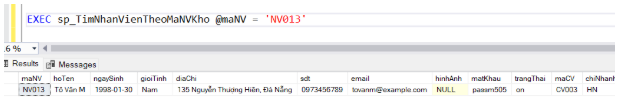
\includegraphics[width=0.8\linewidth]{img/2-5.png}
\end{figure}
\end{document}